\documentclass[spanish,a4paper,14pt,oneside]{extreport}
\usepackage[utf8]{inputenc}
\usepackage[spanish]{babel}
%%%%%%%%%%%%%%%%%%%%%%%%%%%%%%%%%%%%%%%%%%%%%%%%%%%%%%%%%%%%%%%%%%%%%%%%%%%%%%%
% Next 3+3 lines select PDF or PS output respectively (comment as apropriate)
% To switch from PDF and PS comment/uncomment here
% and change correspondingly the Makefile
%
\usepackage[pdftex]{color}
\usepackage[pdftex]{graphicx}
\graphicspath{{FIGURES/}}
%\usepackage[dvips]{color}
%%\usepackage[dvips]{graphicx}
%\graphicspath{{FIGURES/}}
%%%%%%%%%%%%%%%%%%%%%%%%%%%%%%%%%%%%%%%%%%%%%%%%%%%%%%%%%%%%%%%%%%%%%%%%%%%%%%%
\usepackage{alltt}
\usepackage{algorithm}
\usepackage{algorithmic}
\usepackage{multirow}
\usepackage[top=2cm, bottom=2cm, left=2cm, right=2cm]{geometry}
\usepackage{hyperref}

% Símbolo del euro
\usepackage[official]{eurosym}

%%%%%%%%%%%%%%%%%%%%%%%%%%%%%%%%%%%%%%%%%%%%%%%%%%%%%%%%%%%%%%%%%%%%%%%%%%%%%%%

% Referenciar nombres de una lista de items
\makeatletter
\let\orgdescriptionlabel\descriptionlabel
\renewcommand*{\descriptionlabel}[1]{%
  \let\orglabel\label
  \let\label\@gobble
  \phantomsection
  \edef\@currentlabel{#1}%
  %\edef\@currentlabelname{#1}%
  \let\label\orglabel
  \orgdescriptionlabel{#1}%
}
\makeatother

% Indice de referencias cruzadas
\usepackage{makeidx}
\makeindex

%%%%%%%%%%%%%%%%%%%%%%%%%%%%%%%%%%%%%%%%%%%%%%%%%%%%%%%%%%%%%%%%%%%%%%%%%%%%%%%

\newcommand{\SONY}{{\sc Sony}}
\newcommand{\INTEL}{\textsf{\textsc{I}ntel}}

%%% Traducimos el pseudocodigo
\renewcommand{\algorithmicwhile}{\textbf{mientras}}
\renewcommand{\algorithmicend}{\textbf{fin}}
\renewcommand{\algorithmicdo}{\textbf{hacer}}
\renewcommand{\algorithmicif}{\textbf{si}}
\renewcommand{\algorithmicthen}{\textbf{entonces}}
\renewcommand{\algorithmicrepeat}{\textbf{repetir}}
\renewcommand{\algorithmicuntil}{\textbf{hasta que}}
\renewcommand{\algorithmicelse}{\textbf{en otro caso}}
\renewcommand{\algorithmicfor}{\textbf{para}}

%\newcommand{\RETURN}{\textbf{retornar} }
\newcommand{\RET}{\STATE \textbf{retornar} }
\newcommand{\TO}{\textbf{hasta} }
\newcommand{\AND}{\textbf{y} }
\newcommand{\OR}{\textbf{o} }

%Comando para el índice de referencias cruzadas
\newcommand{\cei}[1]
  {\index{#1}\emph{#1}}
  
\newcommand{\ceis}[1]  
  {\index{#1}{\bfseries {#1}}}
  
\newcommand{\ceit}[1]  
  {\index{#1}{#1}}
  
%%%%%%%%%%%%%%%%% Creamos un entorno para listar código fuente %%%%%%%%%%%%%%%
\newenvironment{sourcecode}
{\begin{list}{}{\setlength{\leftmargin}{1em}}\item\scriptsize\bfseries}
{\end{list}}

\newenvironment{littlesourcecode}
{\begin{list}{}{\setlength{\leftmargin}{1em}}\item\tiny\bfseries}
{\end{list}}

\newenvironment{summary}
{\par\noindent\begin{center}\textbf{Abstract}\end{center}\begin{itshape}\par\noindent}
{\end{itshape}}

\newenvironment{keywords}
{\begin{list}{}{\setlength{\leftmargin}{1em}}\item[\hskip\labelsep \bfseries Keywords:]}
{\end{list}}

\newenvironment{palabrasClave}
{\begin{list}{}{\setlength{\leftmargin}{1em}}\item[\hskip\labelsep \bfseries Palabras clave:]}
{\end{list}}

%%%%%%%%%%%%%%%%%%%%%%%%%%%%%%%%%%%%%%%%%%%%%%%%%%%%%%%%%%%%%%%%%%%%%%%%%%%%%%%
\begin{document}
\renewcommand\listtablename{Índice de Tablas}      % Estos comandos (al haber cargado babel)
\renewcommand\listfigurename{Índice de Figuras}    % Han de ir inmediatamente después del begin{document}

%%%%%%%%%%%%%%%%%%%%%%%%%%%%%%%%%%%%%%%%%%%%%%%%%%%%%%%%%%%%%%%%%%%%%%%%%%%%%%%
% First Page
%%%%%%%%%%%%%%%%%%%%%%%%%%%%%%%%%%%%%%%%%%%%%%%%%%%%%%%%%%%%%%%%%%%%%%%%%%%%%%%

\pagestyle{empty}
\thispagestyle{empty}


\newcommand{\HRule}{\rule{\linewidth}{1mm}}
\setlength{\parindent}{0mm}
\setlength{\parskip}{0mm}

\vspace*{\stretch{0.5}}

%\centering{
\includegraphics[width=0.3\textwidth]{images/logo_vertical}                 !!!
\begin{center}
	
\includegraphics[width=0.3\textwidth]{images/logo_vertical}
\end{center}

\vspace*{\stretch{0.5}}
\begin{center}
{\Huge Trabajo de Fin de Máster}
{\Huge Sistemas y Tecnologías Web Aplicadas (SyTWA)}
\end{center}

\HRule
\begin{flushright}
        {\Huge Shell para corrección automática de repositorios de GitHub} \\[2.5mm]
        {\Large \textit{CLI tool for automatic correction of GitHub's repositories} .} \\[5mm]
        {\Large Juan José Labrador González} \\[5mm]


\end{flushright}
\HRule
\vspace*{\stretch{2}}
\begin{center}
  \Large La Laguna, \today
\end{center}

\setlength{\parindent}{5mm}

%%%%%%%%%%%%%%%%%%%%%%%%%%%%%%%%%%%%%%%%%%%%%%%%%%%%%%%%%%%%%%%%%%%%%%%%%%%%%%%
% Signature page (add the official stamp)
%%%%%%%%%%%%%%%%%%%%%%%%%%%%%%%%%%%%%%%%%%%%%%%%%%%%%%%%%%%%%%%%%%%%%%%%%%%%%%%
\newpage
%\cleardoublepage
\thispagestyle{empty}

D. {\bf Casiano Rodríguez León}, con DNI número 42.020.072-S
profesor
Titular de Universidad
adscrito al Departamento
de Ingeniería Informática y de Sistemas
de la Universidad de La Laguna, como tutor

\bigskip
\bigskip
{\bf C E R T I F I C A }

\bigskip
\bigskip
\bigskip
Que la presente memoria titulada:

\bigskip
``{\it Sistemas y Tecnologías Web Aplicadas. Shell para corrección automática de repositorios de GitHub.}''

\bigskip
\bigskip
\bigskip

\noindent ha sido realizada bajo su dirección por D. {\bf Juan José Labrador González},
con DNI número 78.729.778-L.

\bigskip
\bigskip

Y para que así conste, en cumplimiento de la legislación vigente y a los efectos
oportunos firman la presente en La Laguna a \today

%\cleardoublepage
\newpage
%%%%%%%%%%%%%%%%%%%%%%%%%%%%%%%%%%%%%%%%%%%%%%%%%%%%%%%%%%%%%%%%%%%%%%%%%%%%%%%
\thispagestyle{empty}

{ \flushright

\begin{LARGE}
Agradecimientos
\end{LARGE}

\hspace{3mm}

\begin{large}


\hspace{3mm}
La realización de esta asignatura de Trabajo de Fin de Máster no hubiera sido posible sin 
la ayuda de la Sección de Ingeniería Informática de la Escuela Superior de Ingeniería 
y Tecnología, que ha llevado a cabo todos los trámites necesarios.
\bigskip

\hspace{3mm}
Mención especial para mi familia, pareja y amigos, quienes me han alentado para no rendirme y lograr mis objetivos pese a las dificultades y contratiempos encontrados durante la realización de este Trabajo de Fin de Máster.
\bigskip

\hspace{3mm}
Y por último, especialmente agradecer a Casiano Rodríguez León su labor como tutor del 
Trabajo de Fin de Máster. Además de aprender muchísimo junto a él, me ha aconsejado, animado y resuelto mis 
dudas de manera incansable en la realización de este trabajo. Estoy seguro de que la experiencia y conocimientos adquiridos gracias a él, me ayudarán en mis próximos retos profesionales y personales.


\end{large}

}

%%%%%%%%%%%%%%%%%%%%%%%%%%%%%%%%%%%%%%%%%%%%%%%%%%%%%%%%%%%%%%%%%%%%%%%%%%%%%%%%%
\newpage

\begin{huge}
Licencia
\end{huge}

\bigskip
\bigskip
%\centering{
\includegraphics[width=0.2\textwidth]{images/by-nc-sa_88x31}                      !!!
\begin{center}
	
\includegraphics[width=0.2\textwidth]{images/by-nc-sa_88x31}
\end{center}

\begin{center}
{\Large \copyright~Esta obra está bajo una licencia de Creative Commons Reconocimiento-NoComercial-CompartirIgual 4.0 Internacional.
}
\end{center}


%%%%%%%%%%%%%%%%%%%%%%%%%%%%%%%%%%%%%%%%%%%%%%%%%%%%%%%%%%%%%%%%%%%%%%%%%%%%%%%
\newpage  %\cleardoublepage
\begin{abstract}
{\em

El objetivo de este Trabajo de Fin de Máster ha sido integrar los conocimientos adquiridos durante los estudios del Máster y,en especial, del itinerario de Tecnologías de la Información, aproximando al alumno a la resolución de 
problemas de aplicaciones Web y favoreciendo el desarrollo de destrezas propias de la Ingeniería Web: 
se centra en el aprendizaje y puesta en práctica de metodologías, aproximaciones, técnicas y herramientas 
para abordar la creciente complejidad de este tipo de aplicaciones en el marco de las metodologías ágiles. Cada vez ésta cobra más importancia, siendo constante el aumento del número de aplicaciones de escritorio, smartphones y tablets.
\bigskip

En este Trabajo de Fin de Máster se propone el desarrollo de un paquete Node.js (NPM) que facilite la descarga y corrección de repositorios GitHub de alumnos.
Existe un buen número de herramientas de Control de Versiones que permiten alojar proyectos software y agruparlos en organizaciones lógicas, pero carecen de mecanismos para automatizar funciones de uso cotidiano como la descarga de los mismos, la preparación del entorno de cada proyecto o la ejecución de pruebas.
\bigskip

En nuestra propuesta, se ha realizado una primera aproximación a la automatización de descargas y correcciones de repositorios, recopilando todos los datos inherentes de estas acciones y generando los informes correspondientes en formato PDF y HTML. Todo ello mediante un sencillo uso y sentando las bases para proporcionar más funcionalidades a la herramienta en un futuro próximo.
}

\begin{palabrasClave}
Consola, CLI, Shell, Terminal, Node.js, GitHub, Corrección, Automatización
\end{palabrasClave}

\end{abstract}
%%%%%%%%%%%%%%%%%%%%%%%%%%%%%%%%%%%%%%%%%%%%%%%%%%%%%%%%%%%%%%%%%%%%%%%%%%%%%%%

%%%%%%%%%%%%%%%%%%%%%%%%%%%%%%%%%%%%%%%%%%%%%%%%%%%%%%%%%%%%%%%%%%%%%%%%%%%%%%%
\newpage  %\cleardoublepage
\begin{summary}
{\em

The aim of this Master's Degree Final Project has been to integrate all the knowledge gained during the Master studies, especially the knowledge from the Information Technologies speciality, bringing closer to the student the resolution of Web Application's problems and favouring the development of Web Engineering skills. These skills focus on the learning and use of methodologies, technologies and tools to deal with the growing complexity of Web Applications. Those skills are becoming more important, being constant the increase of desktop and mobile applications.
\bigskip

This Master's Degree Final Project proposes the development of a Node.js package (NPM) that facilitates the download and correction of students' GitHub repositories.
There are many Version Control tools that allow to host software projects and group them into logical organizations, but  they haven't automatic methods for downloading them, or setting up the environment for each project and executing tests on them.
\bigskip

In our proposal, we had made a first approach to the automation of repositories' downloads and corrections, gathering all the inherent data of these actions and generating PDF and HTML reports with them. All that through a simple way and setting the bases to provide more functionalities to the tool in a near future.  
}

\begin{keywords}
Console, CLI, Shell, Terminal, Node.js, GitHub, Correction, Automation
\end{keywords}

\end{summary}
%%%%%%%%%%%%%%%%%%%%%%%%%%%%%%%%%%%%%%%%%%%%%%%%%%%%%%%%%%%%%%%%%%%%%%%%%%%%%%%

%%%%%%%%%%%%%%%%%%%%%%%%%%%%%%%%%%%%%%%%%%%%%%%%%%%%%%%%%%%%%%%%%%%%%%%%%%%%%%%
\newpage{\pagestyle{empty}}
\thispagestyle{empty}

%%%%%%%%%%%%%%%%%%%%%%%%%%%%%%%%%%%%%%%%%%%%%%%%%%%%%%%%%%%%%%%%%%%%%%%%%%%%%%%


\pagestyle{myheadings} %my head defined by markboth or markright
% No funciona bien \markboth sin "twoside" en \documentclass, pero al
% ponerlo se dan un montón de errores de underfull \vbox, con lo que no se
% ha puesto.
\markboth{Juan José Labrador González}{Shell para corrección automática de repositorios de GitHub}

%%%%%%%%%%%%%%%%%%%%%%%%%%%%%%%%%%%%%%%%%%%%%%%%%%%%%%%%%%%%%%%%%%%%%%%%%%%%%%%
%Numeracion en romanos
\renewcommand{\thepage}{\roman{page}}
\setcounter{page}{1}

%%%%%%%%%%%%%%%%%%%%%%%%%%%%%%%%%%%%%%%%%%%%%%%%%%%%%%%%%%%%%%%%%%%%%%%%%%%%%%%

\tableofcontents

%%%%%%%%%%%%%%%%%%%%%%%%%%%%%%%%%%%%%%%%%%%%%%%%%%%%%%%%%%%%%%%%%%%%%%%%%%%%%%%
\newpage{\pagestyle{empty}}

\listoffigures

%%%%%%%%%%%%%%%%%%%%%%%%%%%%%%%%%%%%%%%%%%%%%%%%%%%%%%%%%%%%%%%%%%%%%%%%%%%%%%%
\newpage{\pagestyle{empty}}

\listoftables

%%%%%%%%%%%%%%%%%%%%%%%%%%%%%%%%%%%%%%%%%%%%%%%%%%%%%%%%%%%%%%%%%%%%%%%%%%%%%%%
\newpage{\pagestyle{empty}}

%%%%%%%%%%%%%%%%%%%%%%%%%%%%%%%%%%%%%%%%%%%%%%%%%%%%%%%%%%%%%%%%%%%%%%%%%%%%%%%
%Numeracion a partir del capitulo I
\renewcommand{\thepage}{\arabic{page}}
\setcounter{page}{1}


\chapter{Introducción}
\label{chapter:intro}

%%%%%%%%%%%%%%%%%%%%%%%%%%%%%%%%%%%%%%%%%%%%%%%%%%%%%%%%%%%%%%%%%%%%%%%%%%%%%
% Chapter 1: Introducción 
%%%%%%%%%%%%%%%%%%%%%%%%%%%%%%%%%%%%%%%%%%%%%%%%%%%%%%%%%%%%%%%%%%%%%%%%%%%%%%%

%---------------------------------------------------------------------------------
\section{Antecedentes}
\label{1:sec:1}

La \ceit{\ref{apend1:www}} está sujeta a un cambio continuo. La llegada de \ceit{\ref{apend1:html}}, la creciente importancia de \ceit{\ref{apend1:ajax}} y de la programación en el lado del cliente, las nuevas fronteras de la \ceit{\ref{apend1:web}}, y la explosión de las redes sociales son ejemplos de esta tendencia general.
\bigskip

Las aplicaciones web parecen evolucionar hacia entornos cada vez más ricos y flexibles en los que
los usuarios pueden acceder con facilidad a los documentos, publicar contenido, escuchar música, ver
vídeos, realizar dibujos e incluso jugar usando un navegador. Esta nueva clase de software ubicuo no
cesa de ganar momentum y promueve nuevas formas de interacción y cooperación.
\bigskip


Ante la rápida evolución del software, los sistemas de \ceis{\ref{apend1:cvs}} han adquirido una mayor importancia dentro de la metodología del desarrollo del software: la gestión de las versiones del propio software se ha convertido en una actividad crítica. Estos sistemas han evolucionado a la par que el software, proporcionando nuevas funcionalidades y orientándose hacia la colaboración.

%---------------------------------------------------------------------------------
\section{Estado actual del arte}
\label{1:sec:2}

Actualmente, hay numerosos sistemas de control de versiones. Todos ellos proporcionan mecanismos de almacenamiento del código, de modificación y de consulta histórica del mismo, a la vez que proporcionan un entorno colaborativo en el que los usuarios pueden colaborar e interactuar entre sí.

En el caso particular de \ceis{\ref{apend1:github}}, además de proporcionar lo mencionado anteriormente, observando el creciente número de estudiantes que utiliza la plataforma, ha creado herramientas específicas para facilitar sus desarrollos (como por ejemplo \ceit{\ref{apend1:sdp}}) y provee a profesores de herramientas para gestionar dichos desarrollos (como por ejemplo \ceit{\ref{apend1:github-classroom}}).

Sin embargo, estas herramientas de gestión de desarrollos requieren una administración interactiva por parte del profesor. No cuentan aún con funcionalidades de automatización de tareas.

%---------------------------------------------------------------------------------
\section{Objetivos y actividades a realizar}
\label{1:sec:3}

En este proyecto se persigue integrar los conocimientos adquiridos durante los estudios del Máster y,
en especial, del itinerario de Tecnologías de la Información para solucionar problemas actuales de aplicaciones y servicios Web.
\bigskip

Los objetivos propuestos para alcanzar en este Trabajo de Fin de Máster ha sido los siguientes:
\begin{itemize}
  \item Conocer, dominar y practicar con lenguajes y herramientas de desarrollo de aplicaciones Web
en el servidor (\ceis{\ref{apend1:node}}, \ceis{\ref{apend1:npm}}).
  \item Conocer, dominar y practicar con diferentes lenguajes y librerías en el cliente.
  \item Conocer, practicar y dominar herramientas de \ceit{\ref{apend1:tdd}} en entornos web y la Integración Contínua.
  \item Conocer, practicar y dominar diferentes lenguajes de marcas y de estilo.
  \item Conocer, practicar y dominar diferentes mecanismos de despliegue.
  \item Conocer, practicar y familiarizarse con diferentes mecanismos de seguridad, autentificación
y autorización.
  \item Conocer, practicar y dominar diferentes herramientas colaborativas y de control de versiones.
  \item Conocer, practicar y dominar \ceit{\ref{apend1:ma}} de desarrollo de software.
\end{itemize}
\newpage

Y las actividades a realizar en el mismo son las que se describen a continuación:
\begin{itemize}
  \item Revisión bibliográfica y estado del arte.
  \item Desarrollar una herramienta de línea de comandos escrita en {\bfseries Node.js} que permita automatizar tareas relacionadas con \ceit{\ref{apend1:repositorio}} de {\bfseries GitHub}:
  \begin{itemize}
    \item Autenticación con GitHub.
    \item Listar \ceit{\ref{apend1:organizacion}}, \ceit{\ref{apend1:asignaciones}} y repositorios de GitHub del usuario.
    \item Automatizar la descarga de repositorios.
    \item Automatizar la ejecución de scripts en los repositorios (TDD, creación de entorno, evaluación de código...).
    \item Recopilar la información obtenida de la automatización de tareas y presentarla al usuario (PDF, HTML...).
  \end{itemize}
  \item Redacción de la memoria.
  \item Preparación de la presentación oral.
\end{itemize}
\newpage

%---------------------------------------------------------------------------------
\section{Tecnología usada}
\label{1:sec:3}
 
Para llevar a cabo el desarrollo de esta herramienta se planteó realizar el desarrollo en {\bfseries Node.js}, creando una librería modular que se pudiese instalar mediante el gestor de paquetes de Node.js ({\bfseries NPM}).

\begin{figure}[H]
\begin{center}

\includegraphics[width=0.3\textwidth]{images/nodejs-logo}
\end{center}
\end{figure}

Además, se ha hecho uso de otras tecnologías enumeradas a continuación:
\begin{itemize}
  \item \ceit{\ref{apend1:npm}}            
\includegraphics[width=0.15\textwidth]{images/npm}
  \item \ceit{\ref{apend1:github}}         
\includegraphics[width=0.1\textwidth]{images/github}
  \item \ceit{\ref{apend1:gitbook}}        
\includegraphics[width=0.3\textwidth]{images/gitbook}
  \item \ceit{\ref{apend1:travis}}      
\includegraphics[width=0.3\textwidth]{images/travis-ci-logo}
\end{itemize}

%%%%%%%%%%%%%%%%%%%%%%%%%%%%%%%%%%%%%%%%%%%%%%%%%%%%%%%%%%%%%%%%%%%%%%%%%%%%%%%

\chapter{Desarrollo}
\label{chapter:dos}

%%%%%%%%%%%%%%%%%%%%%%%%%%%%%%%%%%%%%%%%%%%%%%%%%%%%%%%%%%%%%%%%%%%%%%%%%%%%%%%
% Chapter 2: Desarrollo
%%%%%%%%%%%%%%%%%%%%%%%%%%%%%%%%%%%%%%%%%%%%%%%%%%%%%%%%%%%%%%%%%%%%%%%%%%%%%%%

%++++++++++++++++++++++++++++++++++++++++++++++++++++++++++++++++++++++++++++++

En el capítulo anterior se ha descrito el estado del arte actual y se ha definido el Trabajo de Fin de Máster, especificado los objetivos, actividades a desarrollar y las tecnologías empleadas para su desarrollo. A continuación, se describirá la metodología de trabajo seguida.

%++++++++++++++++++++++++++++++++++++++++++++++++++++++++++++++++++++++++++++++

\section{Metodología usada}
\label{2:sec:1}

Se ha llevado a cabo una {\it metodología de trabajo ágil}, común en el campo de la Ingeniería Informática, con reuniones periódicas en las que se definían una serie de tareas u objetivos (iteración) y que se presentaban en la siguiente reunión. 
\bigskip

De este modo, con la entrega de prototipos funcionales de la aplicación, se han ido testeando, corrigiendo y mejorando las 
funcionalidades, al mismo tiempo que detectando problemas no contemplados en las fases previas de diseño.
\bigskip

Esta metodología, además, ha propiciado la generación de ideas que se han traducido en nuevas características.
\newpage

%---------------------------------------------------------------------------------
\subsection{GitHub}
\label{subsec:2.1.1}

Para llevar a cabo esta metodología, se ha usado GitHub como herramienta de Control de Versiones (CVS).
Todo el código implementado se alojaba en dicha herramienta, permitiendo así su cómoda modificación y actualización.

\begin{figure}[H]
\begin{center}
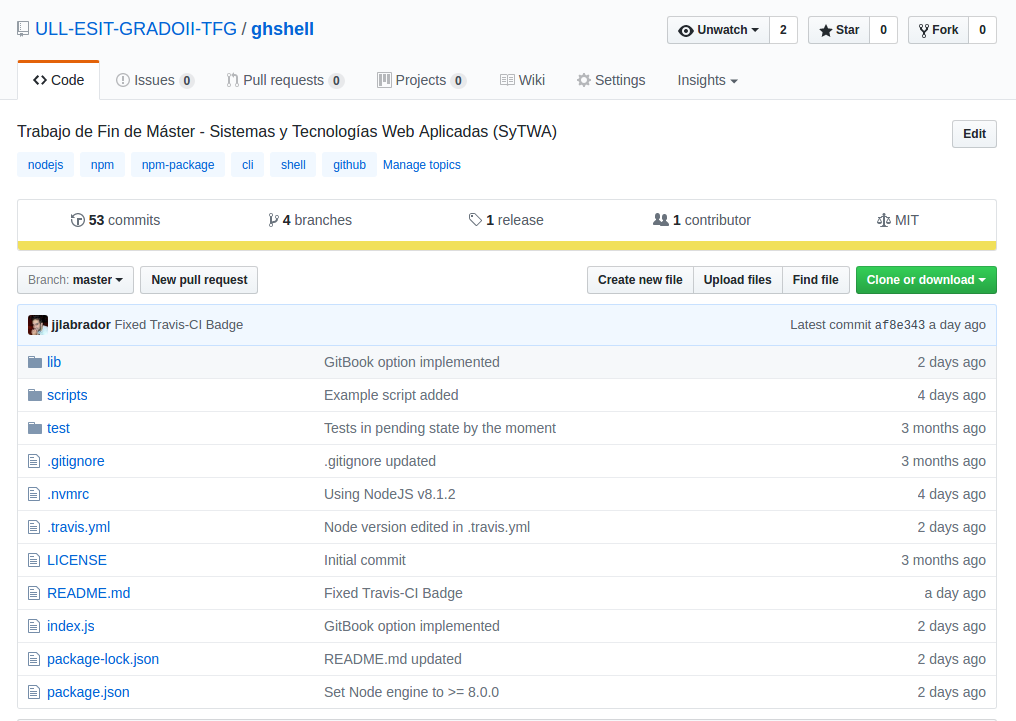
\includegraphics[width=0.9\textwidth]{images/github1}
\caption{Captura del repositorio del paquete NPM en GitHub}
\label{fig:github1}
\end{center}
\end{figure}
\newpage

El trabajo se dividía en ramas, de modo que la versión estable de la aplicación (rama \verb|master|) quedara aislada de la 
versión en desarrollo (rama \verb|develop|) y de la rama experimental (rama \verb|test|).


\begin{figure}[H]
\begin{center}
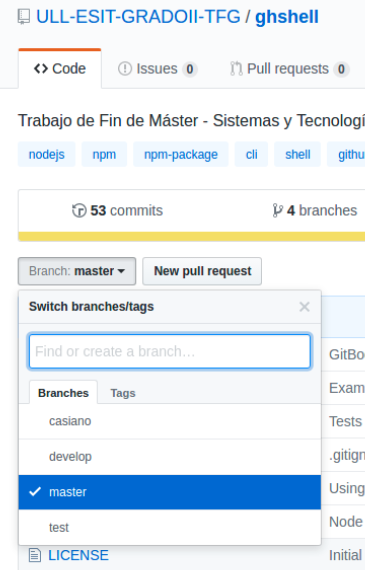
\includegraphics[width=0.47\textwidth]{images/github2}
\caption{Ramas del repositorio}
\label{fig:github2}
\end{center}
\end{figure}
\newpage

La documentación adicional para llevar a cabo los desarrollos de cada iteración, así como los problemas detectados, se anotaban en el apartado de \verb|issues| con el fin de que quedara constancia de ello y se reflejara el estado en el que se encontraba cada uno.

\begin{figure}[H]
\begin{center}
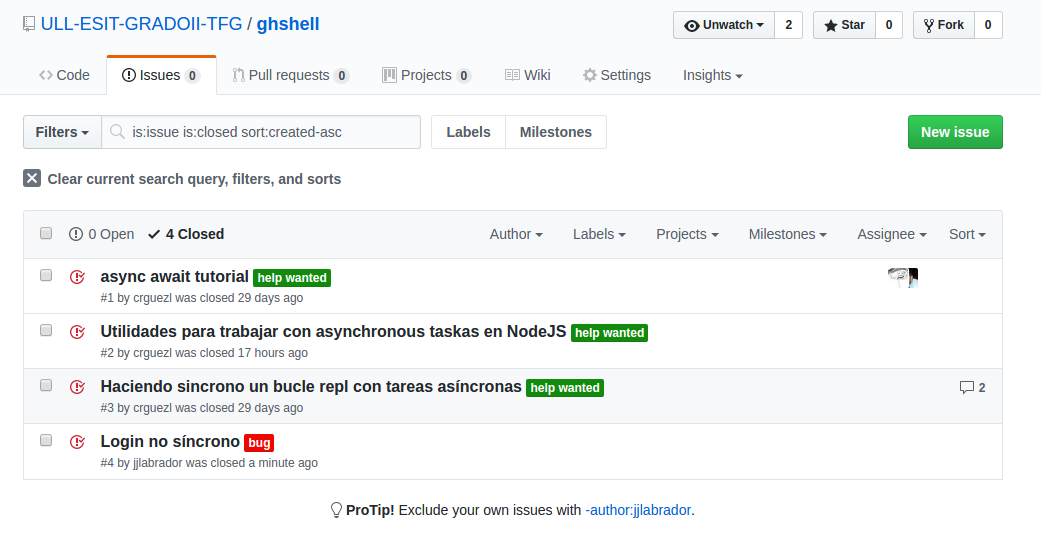
\includegraphics[width=1\textwidth]{images/github3}
\caption{Apartado de issues}
\label{fig:github3}
\end{center}
\end{figure}

%---------------------------------------------------------------------------------
\subsection{Travis-CI}
\label{subsec:2.1.2}

Como herramienta de integración continua, se ha utilizado Travis-CI, con el fin de asegurarnos el despliegue de la aplicación era satisfactorio tras cada cambio subido a la herramienta de control de versiones (GitHub).

\begin{figure}[H]
\begin{center}
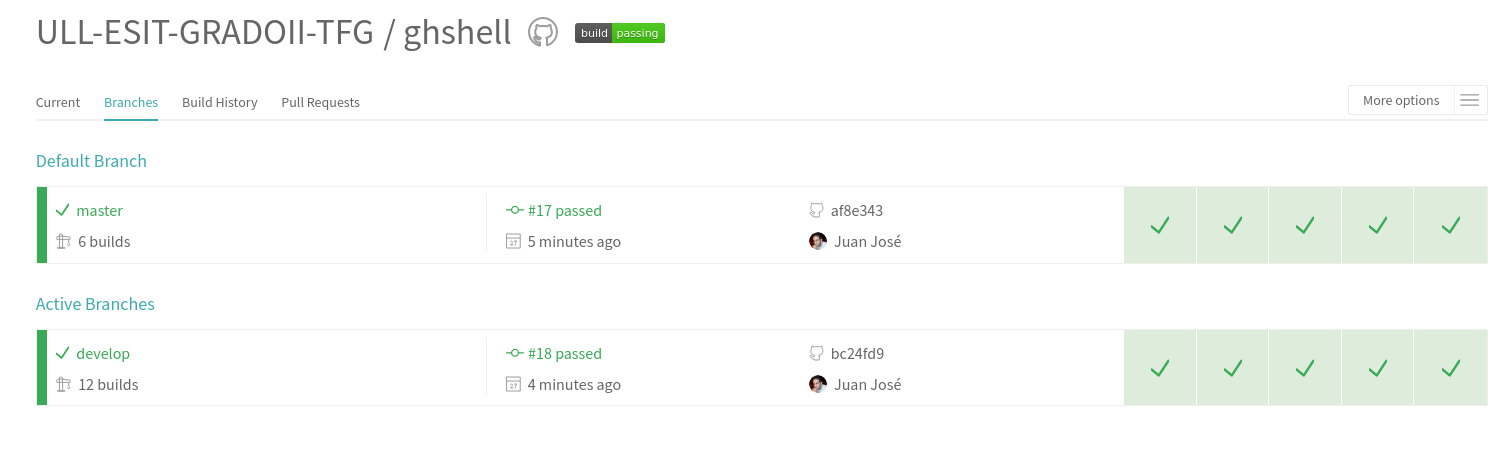
\includegraphics[width=1.1\textwidth]{images/travis-ci}
\caption{Herramienta de integración continua}
\label{fig:travisci}
\end{center}
\end{figure}

%---------------------------------------------------------------------------------
\subsection{Experiencia de usuario}
\label{subsec:2.1.3}

Por otra parte, el tutor del Trabajo de Fin de Máster ha hecho pruebas reales con el resultado de cada iteración, actuando como {\it Product Owner}. 
\bigskip

De este modo, se comprobaba el funcionamiento de la aplicación en un entorno real y se recibía un valioso feedback para corregir problemas o hacer mejoras en las siguientes iteraciones.


%%%%%%%%%%%%%%%%%%%%%%%%%%%%%%%%%%%%%%%%%%%%%%%%%%%%%%%%%%%%%%%%%%%%%%%%%%%%%%%
\newpage{\pagestyle{empty}}
\thispagestyle{empty}

\chapter{Resultados}
\label{chapter:tres}

%%%%%%%%%%%%%%%%%%%%%%%%%%%%%%%%%%%%%%%%%%%%%%%%%%%%%%%%%%%%%%%%%%%%%%%%%%%%%%%
% Chapter 3: Resultados
%%%%%%%%%%%%%%%%%%%%%%%%%%%%%%%%%%%%%%%%%%%%%%%%%%%%%%%%%%%%%%%%%%%%%%%%%%%%%%%

%++++++++++++++++++++++++++++++++++++++++++++++++++++++++++++++++++++++++++++++

Finalizada la etapa de desarrollo del Trabajo de Fin de Máster, se procede a describir la herramienta implementada.


La herramienta se ha denominado \verb|ghhell|, abreviatura de 'GitHub Shell'. Se ha publicado en NPM\cite{URL:NPM} para su fácil distribución e instalación:

\begin{figure}[H]
\begin{center}
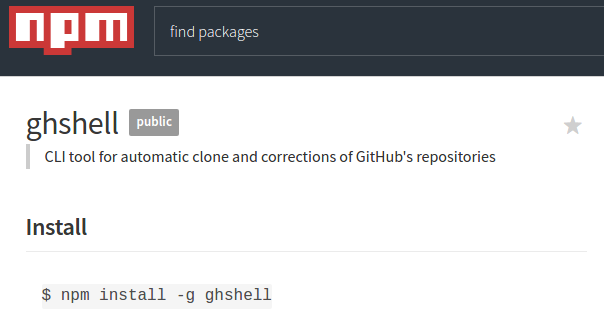
\includegraphics[width=0.8\textwidth]{images/npm1}
\caption{Página del gestor de paquetes NPM}
\label{fig:npm}
\end{center}
\end{figure}

Las funcionalidades implementadas en \verb|ghshell|, se describen a continuación.

%---------------------------------------------------------------------------------
\section{Funcionalidades requeridas}
\label{3:sec:1}

%------------------------------------------------------------------------------------------------------------
\subsection{Autenticación con GitHub}
\label{subsec:3.1.1}
    
    Una vez que el usuario se autentifica con GitHub, se genera un token personal, que se usa posteriormente para acceder a la API de Github. Este token se almacena cifrado en el equipo del usuario, por lo que las siguientes ocasiones que utilice la herramienta no hará falta que vuelva a iniciar sesión:
        
        \begin{figure}[H]
		\begin{center}
		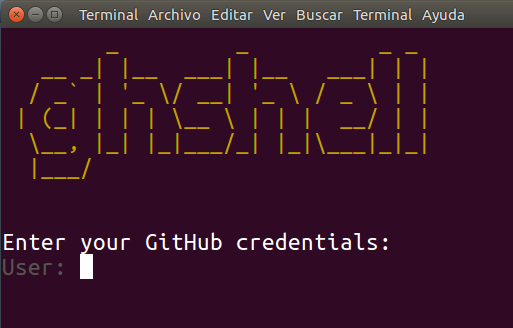
\includegraphics[width=0.7\textwidth]{images/ghshell1}
		\caption{Login de usuario}
		\label{fig:ghshell1}
		\end{center}
		\end{figure}
		
		\begin{figure}[H]
		\begin{center}
		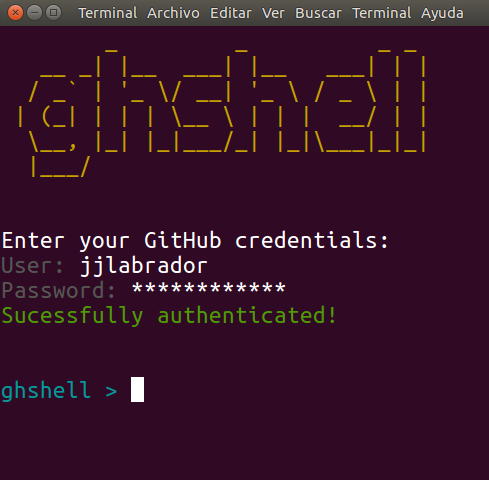
\includegraphics[width=0.6\textwidth]{images/ghshell2-1}
		\caption{Usuario autenticado}
		\label{fig:ghshell2-1}
		\end{center}
		\end{figure}
		
		\begin{figure}[H]
		\begin{center}
		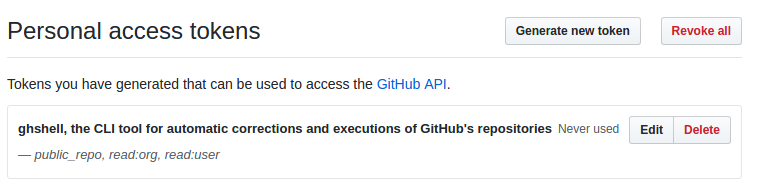
\includegraphics[width=1\textwidth]{images/ghshell2-3}
		\caption{Token personal en GitHub}
		\label{fig:ghshell2-3}
		\end{center}
		\end{figure}
		
		\begin{figure}[H]
		\begin{center}
		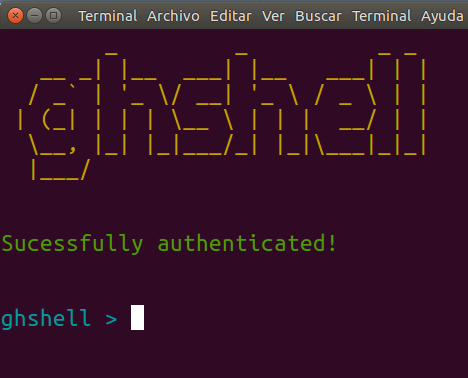
\includegraphics[width=0.6\textwidth]{images/ghshell2-4}
		\caption{Login automático una vez generado el token}
		\label{fig:ghshell2-4}
		\end{center}
		\end{figure}
		
	Si el usuario cierra sesión en la herramienta, se eliminará el token en GitHub y en el equipo:
	
		\begin{figure}[H]
		\begin{center}
		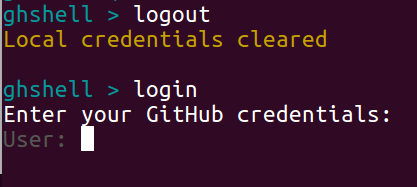
\includegraphics[width=0.6\textwidth]{images/ghshell2-2}
		\caption{Logout de usuario}
		\label{fig:ghshell2-2}
		\end{center}
		\end{figure}

%------------------------------------------------------------------------------------------------------------
\subsection{Listar organizaciones, asignaciones y repositorios de GitHub del usuario}
\label{subsec:3.1.2}   
    
    Con el comando \verb|'orgs -l'|, se puede listar las organizaciones del usuario y usando \verb|'repos -l'|, se listarán los repositorios del usuario. También se puede acceder 'virtualmente' a las organizaciones y listar los repositorios que contiene, así como las asignaciones.
    
    Las asignaciones son un conjunto de repositorios que corresponden a una tarea asignada por los profesores a los alumnos.
\bigskip

    NOTA: se puede consultar toda la información referente a los comandos del programa en el Apéndice 2.
        
        \begin{figure}[H]
		\begin{center}
		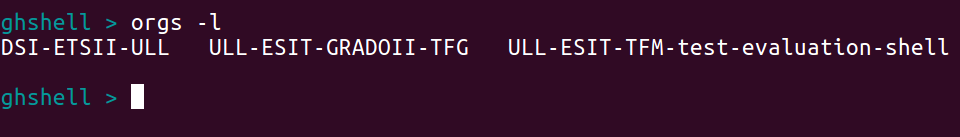
\includegraphics[width=0.9\textwidth]{images/ghshell3}
		\caption{Lista de organizaciones del usuario}
		\label{fig:ghshell3}
		\end{center}
		\end{figure}
		
		\begin{figure}[H]
		\begin{center}
		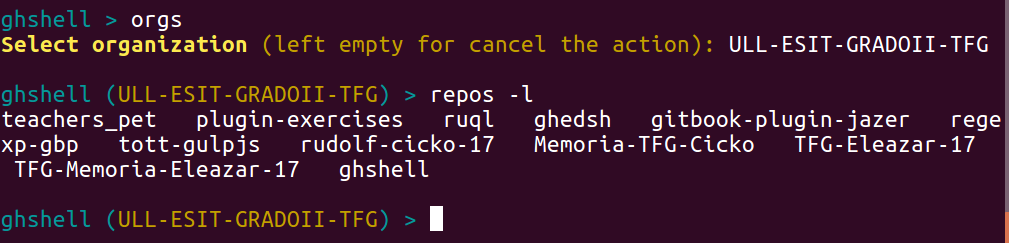
\includegraphics[width=0.9\textwidth]{images/ghshell4}
		\caption{Lista de repositorios de una organización}
		\label{fig:ghshell4}
		\end{center}
		\end{figure}
		
		\begin{figure}[H]
		\begin{center}
		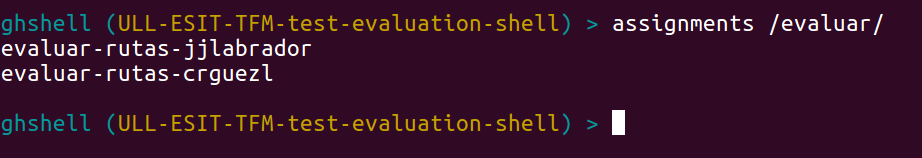
\includegraphics[width=0.9\textwidth]{images/ghshell5}
		\caption{Asignaciones dentro de otra organización}
		\label{fig:ghshell5}
		\end{center}
		\end{figure}
		
	También es posible acceder 'virtualmente' a los repositorios y realizar acciones sobre ellos:
	
		\begin{figure}[H]
		\begin{center}
		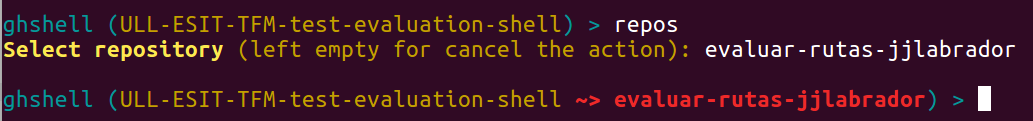
\includegraphics[width=1\textwidth]{images/ghshell5-1}
		\caption{Acceso a un repositorio de una organización}
		\label{fig:ghshell5-1}
		\end{center}
		\end{figure}

%------------------------------------------------------------------------------------------------------------
\subsection{Automatizar la descarga de repositorios}
\label{subsec:3.1.3}  
        	
    En función del contexto dónde nos encontremos dentro de la herramienta, podremos:
    \begin{itemize}
    	\item Clonar el repositorio en el que nos encontremos.
    	\item Clonar un repositorio determinado.
	    \item Clonar todos los repositorios que coincidan con una determinada expresión regular.
	    \item Clonar todos los repositorios de una asignación que coincidan con una determinada expresión
    \end{itemize}
    
    El clonado se realiza de manera asíncrona, por lo que podemos seguir trabajando mientras se clona(n) el/los repositorio(s). Se puede observar el estado de la clonación revisando el fichero de log que se genera cuyo nombre sigue el formato: \textless \verb|nombre-repositorio|\textgreater \verb|-clone.log|.
    
    	\begin{figure}[H]
		\begin{center}
		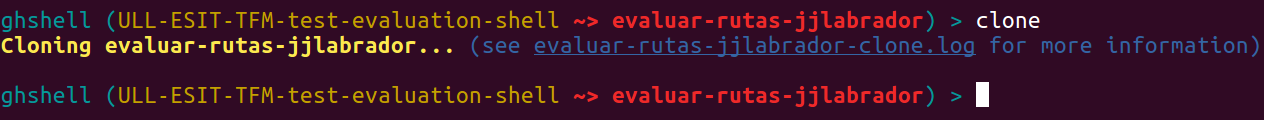
\includegraphics[width=1\textwidth]{images/ghshell6-3}
		\caption{Clonado del repositorio donde nos encontramos}
		\label{fig:ghshell6-3}
		\end{center}
		\end{figure}	

    Si clonamos repositorios que pertenecen a una organización, se creará una carpeta con el nombre de la organización y en su interior se guardarán los repositorios clonados.
    		
	Además, si clonamos repositorios que pertenecen a una asignación, también se creará una carpeta con el nombre de la asignación que los contendrá.
	
        \begin{figure}[H]
		\begin{center}
		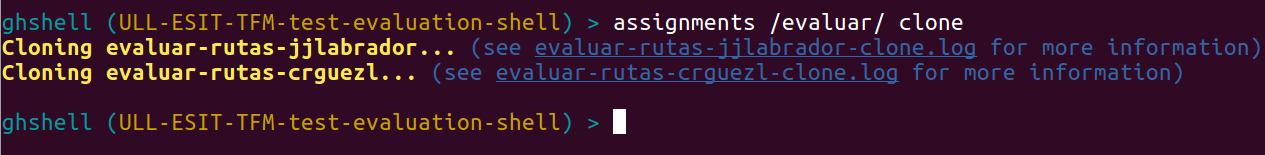
\includegraphics[width=1\textwidth]{images/ghshell6-1}
		\caption{Clonado de asignaciones que coinciden con una expresión regular}
		\label{fig:ghshell6-1}
		\end{center}
		\end{figure}	
		
		\begin{figure}[H]
		\begin{center}
		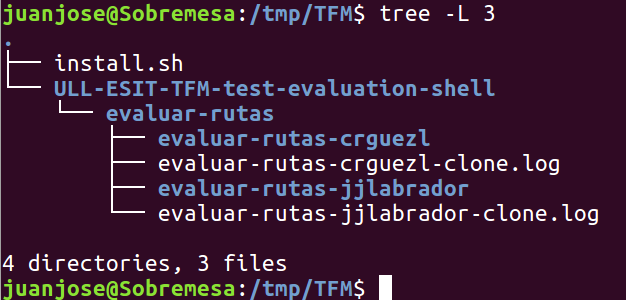
\includegraphics[width=0.7\textwidth]{images/ghshell6-2}
		\caption{Resultado del clonado}
		\label{fig:ghshell6-2}
		\end{center}
		\end{figure}
	
%------------------------------------------------------------------------------------------------------------
\subsection{Automatizar la ejecución de scripts en los repositorios}
\label{subsec:3.1.3} 
	    
    En función del contexto donde nos encontremos dentro de la herramienta, podremos:
    \begin{itemize}
    	\item Ejecutar un script en el repositorio en el que nos encontremos.
    	\item Ejecutar un script en un determinado repositorio.
	    \item Ejecutar un script en todos los repositorios que coincidan con una determinada expresión regular.
	    \item Ejecutar un script en todos los repositorios de una asignación coincidan con una determinada expresión regular.
    \end{itemize}
    
	La ruta del fichero del script puede ser absoluta o relativa. Estos scripts puede ser de cualquier tipo: TDD, creación de entorno, evaluación de código...
\bigskip

	La ejecución de cada script se ejecuta en un proceso hijo independiente pero, a diferencia del clonado, el script se ejecuta línea a línea de manera síncrona. Se puede observar el estado de la ejecución del script y los resultados revisando el fichero de log que se genera: \textless nombre-repositorio \textgreater - \textless nombre-script \textgreater .log
    	
    	\begin{figure}[H]
		\begin{center}
		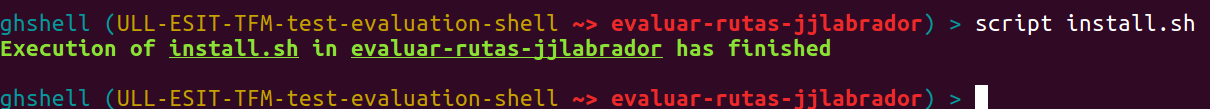
\includegraphics[width=1\textwidth]{images/ghshell7-3}
		\caption{Ejecución del script 'install.sh' en el repositorio actual}
		\label{fig:ghshell7-3}
		\end{center}
		\end{figure}
		
        \begin{figure}[H]
		\begin{center}
		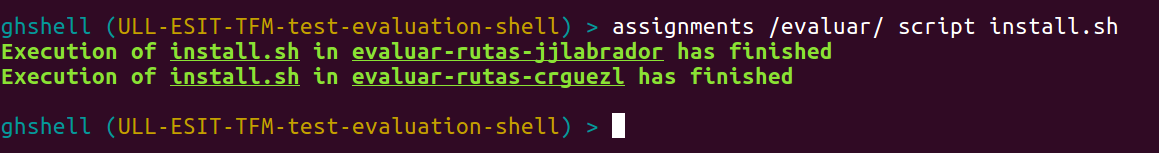
\includegraphics[width=1\textwidth]{images/ghshell7-1}
		\caption{Ejecución del script 'install.sh' en asignaciones que coinciden con una expresión regular}
		\label{fig:ghshell7-1}
		\end{center}
		\end{figure}	
		
		\begin{figure}[H]
		\begin{center}
		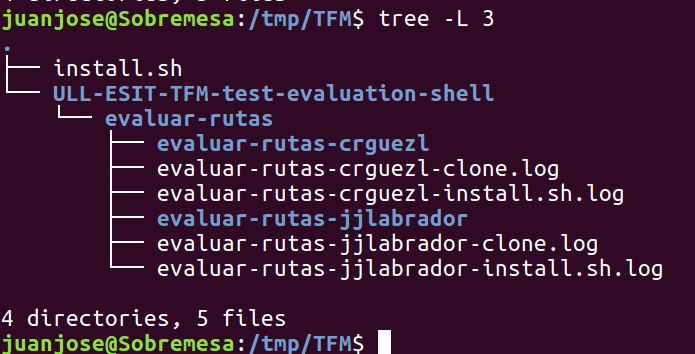
\includegraphics[width=0.7\textwidth]{images/ghshell7-2}
		\caption{Resultado de la ejecución del script 'install.sh'}
		\label{fig:ghshell7-2}
		\end{center}
		\end{figure}
		
%------------------------------------------------------------------------------------------------------------
\subsection{Recopilar la información obtenida de la automatización de tareas}
\label{subsec:3.1.4}

    Una vez ejecutados los scripts necesarios para evaluar un determinado repositorio, es posible generar un GitBook con el resultado de la ejecución de los mismos. Este libro se genera en formato PDF y en HTML.
\bigskip
    
    En función del contexto dónde nos encontremos dentro de la herramienta, podremos:
    \begin{itemize}
    	\item Crear un GitBook en el repositorio en el que nos encontremos.
    	\item Crear un GitBook en un determinado repositorio.
	    \item Crear un GitBook en todos los repositorios que coincidan con una determinada expresión regular.
	    \item Crear un GitBook en todos los repositorios de una asignación coincidan con una determinada expresión regular.
    \end{itemize}
        
        \begin{figure}[H]
		\begin{center}
		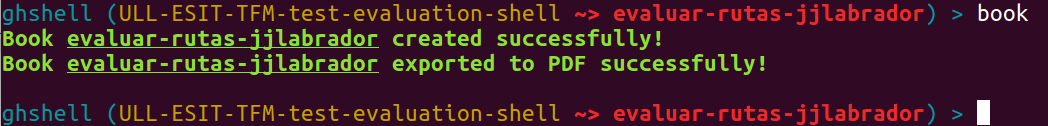
\includegraphics[width=1\textwidth]{images/ghshell8-3}
		\caption{Creación del Gitbook en el repositorio actual}
		\label{fig:ghshell8-3}
		\end{center}
		\end{figure}
		
        \begin{figure}[H]
		\begin{center}
		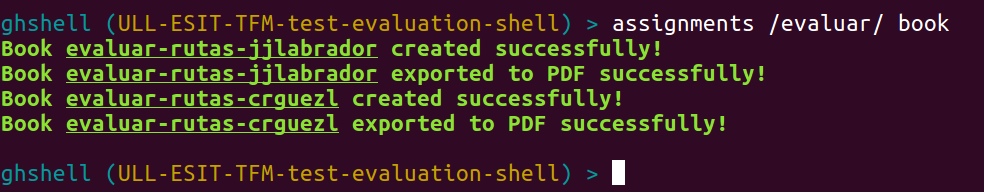
\includegraphics[width=1\textwidth]{images/ghshell8-1}
		\caption{Creación del Gitbook en asignaciones que coinciden con una expresión regular}
		\label{fig:ghshell8-1}
		\end{center}
		\end{figure}	
		
		\begin{figure}[H]
		\begin{center}
		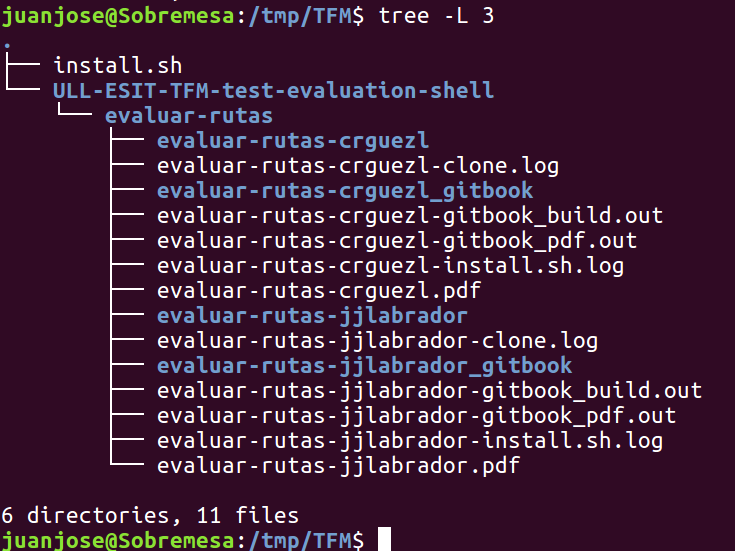
\includegraphics[width=0.7\textwidth]{images/ghshell8-2}
		\caption{Resultado de la creación del Gitbook}
		\label{fig:ghshell8-2}
		\end{center}
		\end{figure}
		
        		        		[ Imagen HTML]
        		        		        		[ Imagen PDF]
\newpage
%---------------------------------------------------------------------------------
\section{Funcionalidades extra}
\label{3:sec:2}

Además de las funcionales solicitadas en este Trabajo de Fin de Máster, se han añadido una serie de funcionalidades extra que, a pesar de no ser requeridas, brindan al usuario de una mejor experiencia de uso del programa:

\begin{itemize}
	\item Autocompletado de los comandos disponibles, pulsando tabulador, en función del contexto donde nos encontremos (nivel principal, organización o repositorio):
	
		\begin{figure}[H]
		\begin{center}
		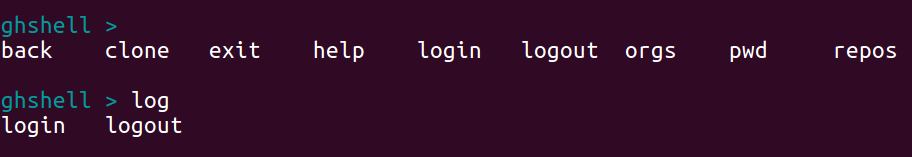
\includegraphics[width=1\textwidth]{images/tab1-1}
		\caption{Autocompletado de comandos}
		\label{fig:tab1-1}
		\end{center}
		\end{figure}
	
	
	Además, también es posible autocompletar los nombres de las organizaciones y repositorios, haciendo mucho más fácil su escritura:
	
		\begin{figure}[H]
		\begin{center}
		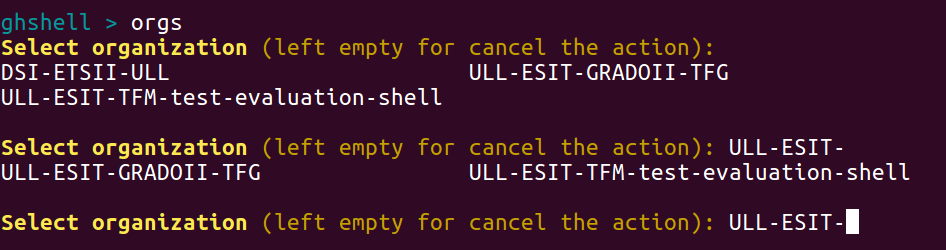
\includegraphics[width=1\textwidth]{images/tab1-2}
		\caption{Autocompletado de organizaciones}
		\label{fig:tab1-1}
		\end{center}
		\end{figure}
		
		\begin{figure}[H]
		\begin{center}
		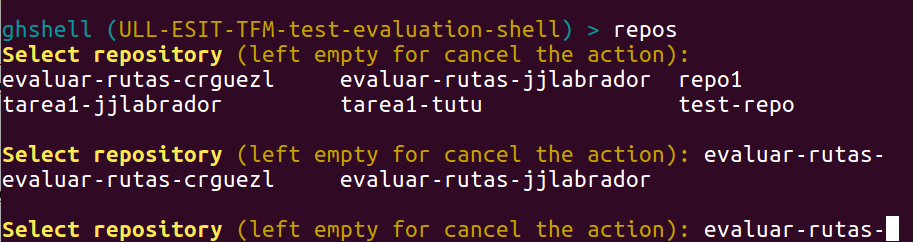
\includegraphics[width=1\textwidth]{images/tab1-3}
		\caption{Autocompletado de repositorios}
		\label{fig:tab1-1}
		\end{center}
		\end{figure}
	
	\item Opción de ayuda que muestra la descripción de los comandos y cómo se utilizan. Esta ayuda varía dependiendo del contexto donde nos encontremos:
	
		\begin{figure}[H]
		\begin{center}
		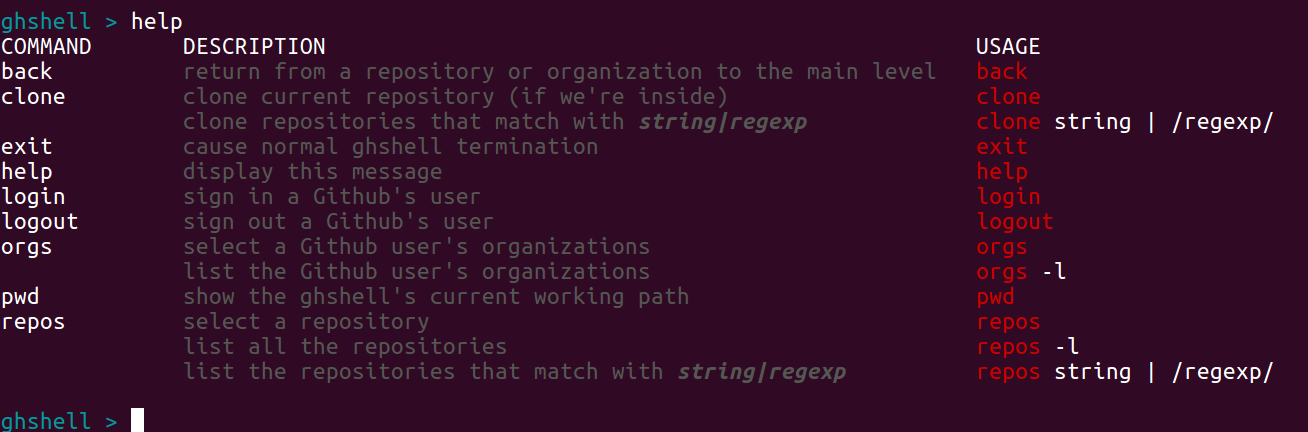
\includegraphics[width=1\textwidth]{images/help1-1}
		\caption{Ayuda global}
		\label{fig:help1-1}
		\end{center}
		\end{figure}
		
		\begin{figure}[H]
		\begin{center}
		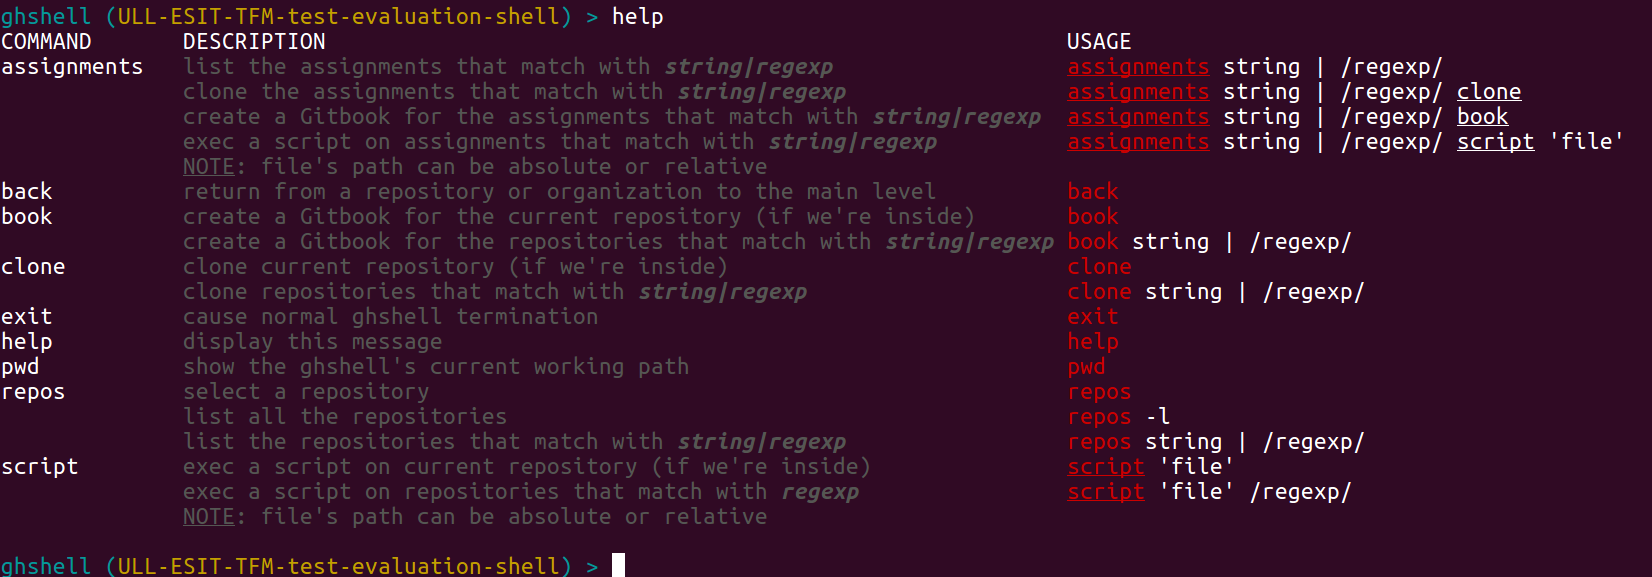
\includegraphics[width=1\textwidth]{images/help1-2}
		\caption{Ayuda en el contexto de organización}
		\label{fig:help1-2}
		\end{center}
		\end{figure}
	
	\item Opción de visualizar el directorio de trabajo donde se ha ejecutado el programa. Útil para determinar rutas relativas de los scripts que se desean ejecutar.
	
		\begin{figure}[H]
		\begin{center}
		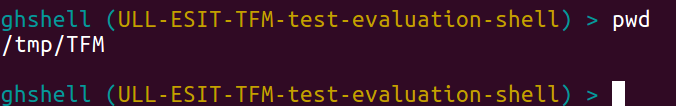
\includegraphics[width=0.7\textwidth]{images/pwd}
		\caption{Directorio actual de trabajo}
		\label{fig:pwd}
		\end{center}
		\end{figure}
	
	
	\item Opción para conocer el propietario de cada repositorio. En el caso de que el repositorio pertenezca a una organización, mostrará los contribuyentes de ese repositorio.
\end{itemize}

		\begin{figure}[H]
		\begin{center}
		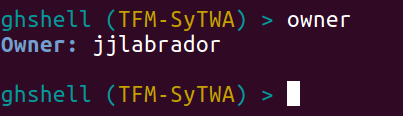
\includegraphics[width=0.5\textwidth]{images/owner1-1}
		\caption{Propietario del repositorio}
		\label{fig:owner1-1}
		\end{center}
		\end{figure}
		
		\begin{figure}[H]
		\begin{center}
		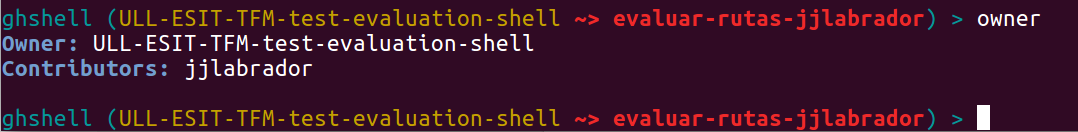
\includegraphics[width=1\textwidth]{images/owner1-2}
		\caption{Contribuyentes del repositorio}
		\label{fig:owner1-2}
		\end{center}
		\end{figure}
	
NOTA: se puede consultar toda la información referente a los comandos del programa en el Apéndice 2.

%---------------------------------------------------------------------------------
\section{Problemas encontrados y soluciones}
\label{3:sec:3}

A continuación se detallan los problemas encontrados durante la implementación de la herramienta y las soluciones encontradas para los mismos:

%---------------------------------------------------------------------------------
\subsection{Asincronía}
\label{subsec:3.3.1}

Una de las características más importantes del lenguaje JavaScript es la asincronía. Usa un modelo de operaciones de entrada/salida sin bloqueo y orientado a eventos, que lo hace ligero y eficiente. Sin embargo, algunas acciones que debía realizar esta herramienta debían de ser síncronas. Ejemplos son el login del usuario y ejecución de scripts.
\bigskip

{\normalsize {\bfseries Solución}}
\bigskip

La solución a este comportamiento pasó por realizar un amplio estudio de la documentación para usar mecanismos que permitieran bloquear la ejecución de la herramienta en las partes que deseábamos. Los mecanismos usados han sido:

\begin{itemize}
	\item Funciones síncronas del propio lenguaje.
	\item Promesas
	\item Métodos async/await
	\item Librerías con métodos implementados de manera síncrona.
\end{itemize}

%---------------------------------------------------------------------------------
\subsection{Autocompletado de comandos}
\label{subsec:3.3.2}

Para el manejo de los flujos de lectura y escritura estándar de la herramienta, se ha utilizado la interfaz nativa de Node.js (Readline). Esta interfaz provee de una función de autocompletado para el texto que escribe el usuario.

Sin embargo, sólo funciona con la primera palabra (comando) que escribe. Tras investigar al respecto y buscar posibles librerías alternativas, no existía ninguna solución que corrigiera este comportamiento.
\bigskip

{\normalsize {\bfseries Solución}}
\bigskip

Realizando numerosas pruebas, se halló una manera propia de conseguir completar más de un comando en la misma línea. Cuando realice los test de aceptación pertinentes requeridos por la comunidad de Node, solicitaré un Pull Request a su repositorio con esta mejora.


%---------------------------------------------------------------------------------
\section{Perfil del usuario de ghshell}
\label{3:sec:4}

El uso de \verb|ghshell| está especialmente dirigido a un determinado grupo de profesores: nos referimos al perfil de un profesor, principalmente docente en alguna rama de Ingeniería, con conocimientos avanzados en programación y en herramientas de control de versiones.

No obstante, ya que la curva de aprendizaje de \verb|ghshell| no es excesiva y dado que el uso de las herramientas de control de versiones no se limita exclusivamente a repositorios de código fuente, se puede extender su uso para el resto de profesorado y usuarios con otros roles. Basta con tener claras unas nociones básicas de informática, junto con la lectura y asimilación previa de la documentación de la herramienta.


%%%%%%%%%%%%%%%%%%%%%%%%%%%%%%%%%%%%%%%%%%%%%%%%%%%%%%%%%%%%%%%%%%%%%%%%%%%%%%%
\newpage{\pagestyle{empty}}
\thispagestyle{empty}

\chapter{Conclusiones y líneas futuras}
\label{chapter:Conclusiones}

%%%%%%%%%%%%%%%%%%%%%%%%%%%%%%%%%%%%%%%%%%%%%%%%%%%%%%%%%%%%%%%%%%%%%%%%%%%%%
% Chapter 4: Conclusiones y Trabajos Futuros 
%%%%%%%%%%%%%%%%%%%%%%%%%%%%%%%%%%%%%%%%%%%%%%%%%%%%%%%%%%%%%%%%%%%%%%%%%%%%%%%

%++++++++++++++++++++++++++++++++++++++++++++++++++++++++++++++++++++++++++++++

Desde hace unos años hasta ahora, ha tenido lugar un enorme crecimiento de las herramientas de control de versiones. Se han convertido en una herramienta imprescindible en la metodologías de desarrollo del software y las instituciones de enseñanza saben que incorporarlas a sus sistemas educativos es clave para ofrecer un servicio puntero y de calidad.
\bigskip

Ésto es lo que se pretende con la herramienta obtenida tras la realización de este Trabajo de Fin de Máster: que sea posible su implantación dentro del marco académico de la Universidad de La Laguna, partiendo de la premisa de que, actualmente, el desarrollo de un proyecto software sin tener detrás un sistema de control de versiones, no es viable.
\bigskip

La automatización de las tareas de clonado y ejecución de pruebas facilitaría al profesor, en primera instancia, la corrección de las prácticas y proyectos de los alumnos. El ahorro de tiempo de ejecutar estas tareas manualmente es considerable, teniendo en cuenta el número de prácticas que realiza cada alumno por asignatura. Esta enorme carga de trabajo del profesor puede ser aprovechada en otros ámbitos docentes.
\bigskip

Por otra parte, esta herramienta sienta las bases a posibles desarrollos futuros, ampliando las funcionalidades de la misma. Se ha desarrollado pensando en su posible escalabilidad y ya que cuenta con toda la estructura base creada (autentificación de usuarios, clonado, ejecución y reporte de resultados), se pueden añadir funcionalidades sin demasiado esfuerzo.
\newpage

Para concluir, podemos afirmar que los objetivos marcados al comienzo de este Trabajo de Fin de Máster han sido cumplidos y las principales líneas de desarrollo a continuar podrían ser las enumeradas a continuación:  

\begin{itemize}
	\item Generar scripts en \verb|Bash| para evaluar aplicaciones (instalación de dependencias, comprobación de calidad de código y ejecución de tests) en varios lenguajes: \verb|Node.js|, \verb|C++|, \verb|Ruby|, \verb|Python|, etc.
	\bigskip
	
	Esta colección de scripts podrían formar parte de la distribución o bien ser distribuidos separadamente como aplicaciones que facilitan el uso de \verb|ghshell|.
	
	\item Dar soporte a la ejecución de scripts escritos en otros lenguajes: Ruby, Python...
	\item Generar {\it issues} en cada repositorio con los resultados de los scripts que se ejecuten.
	\item Crear {\it ramas} en cada repositorio con los resultados de los scripts.
\end{itemize}

%%%%%%%%%%%%%%%%%%%%%%%%%%%%%%%%%%%%%%%%%%%%%%%%%%%%%%%%%%%%%%%%%%%%%%%%%%%%%%%
\newpage{\pagestyle{empty}}
\thispagestyle{empty}

\chapter{Summary and Conclusions }
\label{chapter:ingles}

%%%%%%%%%%%%%%%%%%%%%%%%%%%%%%%%%%%%%%%%%%%%%%%%%%%%%%%%%%%%%%%%%%%%%%%%%%%%%
% Chapter 5: Summary and Conlusions
%%%%%%%%%%%%%%%%%%%%%%%%%%%%%%%%%%%%%%%%%%%%%%%%%%%%%%%%%%%%%%%%%%%%%%%%%%%%%%%

%++++++++++++++++++++++++++++++++++++++++++++++++++++++++++++++++++++++++++++++

From a few years to now, it has had a enourmous growth of Version Control tools. It has become in an indispensable tool in the software development methodologies and all the teaching institutions know that incorporing them to their education systems is fundamental to providing a quality service.
\bigskip

This is what is intended with the developed tool after the completion of this Master's Degree Final Project: that it would be deployed at University of La Laguna basing on the premise that, currently, the development of a software project without using a version control system, is not viable. 
\bigskip

The automation of cloning and execution tasks would facilitate, in first instance, the students' projects correction. The amount of saved time per the teacher is considarable, keeping in mind the large amount of practices of each student per subject. This huge teacher's workload could be use in another academic scopes.
\bigskip

By the other hand, this tool set the bases to future improvements, like enlarge their own functionalities. It has been developed thinking about the scalability and, as it has all the structure created (user's authentication, cloning, execution and reporting), it's possible to add improvements without too effort.
\newpage

In conclusion, we can affirm that all the goals established at the beggining of the subject have been fulfilled and the next development guidelines could be:


\begin{itemize}
	\item Create scripts in \verb|Bash| to evaluate applications (installation of dependencies, code quality check and running tests) in several programming languages: \verb|Node.js|, \verb|C++|, \verb|Ruby|, \verb|Python|, etc.
	\bigskip
	
	This collections of scripts may be incorporated in the tool distribution or be supplied as standalone's applications which facilitate the use of \verb|ghshell|.
	
	\item Provide support to execute scripts written in anothers programming languages: Ruby, Python...
	\item Create {\it issues} in repositories with the results of scripts' executions.
	\item Create branches in repositories with the results of scripts' executions.
\end{itemize}


%%%%%%%%%%%%%%%%%%%%%%%%%%%%%%%%%%%%%%%%%%%%%%%%%%%%%%%%%%%%%%%%%%%%%%%%%%%%%%%
\newpage{\pagestyle{empty}}
\thispagestyle{empty}

\chapter{Presupuesto}
\label{chapter:presupuesto}

\input{cap6.tex}

%%%%%%%%%%%%%%%%%%%%%%%%%%%%%%%%%%%%%%%%%%%%%%%%%%%%%%%%%%%%%%%%%%%%%%%%%%%%%%%
\newpage{\pagestyle{empty}}
\thispagestyle{empty}
\begin{appendix}

\chapter{Glosario}
\label{appendix:1}
{\bfseries {\Huge A}}\label{Apendice1:A}
\bigskip
\bigskip

\begin{description}
  \item[\underline{AJAX}\label{apend1:ajax}]: acrónimo de \textit{Asynchronous JavaScript And XML} (JavaScript asíncrono y XML). Es una técnica de desarrollo web para crear aplicaciones interactivas o RIA (\textit{Rich Internet Applications}). Estas aplicaciones se ejecutan en el cliente, es decir, en el navegador de los usuarios mientras se 
  mantiene la comunicación asíncrona con el servidor en segundo plano. De esta forma es posible realizar cambios sobre las páginas sin necesidad de recargarlas, mejorando la interactividad, velocidad y usabilidad en las aplicaciones.
  \bigskip
\end{description}

\begin{description}
  \item[\underline{API}\label{apend1:api}]: (\textit{Application Programming Interface} o Interfaz de Programación de Aplicaciones). Conjunto de funciones y procedimientos o métodos que ofrece cierta librería para ser utilizados por otro software como una capa de abstracción. 
  \bigskip
\end{description}

\begin{description}
  \item[\underline{asincrona}\label{apend1:asincrona}]: manera en la que una función de un lenguaje de programación ejecuta instrucciones sin causar bloqueos. No espera que finalice la ejecución de la primera instrucción para continuar con la siguiente.
  \bigskip
\end{description}

\begin{description}
  \item[\underline{Asignaciones}\label{apend1:asignaciones}]: conjunto de repositorios que corresponden a una tarea asignada por los profesores a los alumnos. Se configura desde GitHub Classroom usando un repositorio como plantilla y genera copias del mismo a todo aquel que acepte esa asignación. Las asignaciones se comparten mediante enlaces.
  \bigskip
\end{description}

\begin{description}
  \item[\underline{Async/Await}\label{apend1:async-await}]: funcionalidad de Node.js introducida a partir de la versión 7.6 que evita la anidación de callbacks o secuencias de operaciones asíncronas. Permite serializar el código como una secuencia de operaciones síncronas.
  \bigskip
\end{description}


\bigskip
\bigskip
{\bfseries {\Huge C}}\label{Apendice1:C}
\bigskip
\bigskip

\begin{description}
  \item[\underline{Callback}\label{apend1:callback}]: función que se usa como argumento de otra y que se ejecuta cuando se invoca ésta última. 
  \bigskip
\end{description}

\begin{description}
   \item[\underline{Control de Versiones}\label{apend1:cvs}]: (\textit{Control Versioning System} o CVS). Aplicación informática que implementa un sistema de control de versiones: mantiene el registro de todo el trabajo y los cambios en los ficheros (código fuente principalmente) que forman un proyecto y permite la colaboración entre distintos desarrolladores.
  \bigskip
\end{description}


{\bfseries {\Huge G}}\label{Apendice1:G}
\bigskip
\bigskip

\begin{description}
  \item[\underline{GitBook}\label{apend1:gitbook}]: herramienta que permite elaborar documentación de manera rápida usando Markdown como lenguaje de marcado. Esta documentación se puede publicar de manera online como página web o generar Ebooks (en formato ePub, Mobi o PDF). Además, se integra fácilmente con el sistema de control de versiones de GitHub. Para más información, visitar {\small \url{https://www.gitbook.com}}.
  \bigskip
\end{description}

\begin{description}
  \item[\underline{GitHub}\label{apend1:github}]: forja para alojar proyectos utilizando el Sistema de Control de Versiones {\bfseries Git}. Para más información, visitar {\small \url{https://github.com}}.
  \bigskip
\end{description}

\begin{description}
  \item[\underline{GitHub Classroom}\label{apend1:github-classroom}]: herramienta de GitHub que automatiza la creación de repositorios y el control de acceso a ellos, distribuyendo el código inicial de manera sencilla y mostrando las asignaciones que se han creado. Para más información, visitar {\small \url{https://classroom.github.com/}}.
  \bigskip
\end{description}

\bigskip
{\bfseries {\Huge H}}\label{Apendice1:H}
\bigskip
\bigskip

\begin{description}
  \item[\underline{HTML5}\label{apend1:html}]: (\textit{HyperText Markup Language}). Lenguaje de marcado para la elaboración de páginas web. Es un estándar que sirve de referencia para la elaboración de páginas web definiendo una estructura básica y un código para la definición del contenido de la misma.
  \bigskip
\end{description}

\bigskip
\newpage

{\bfseries {\Huge J}}\label{Apendice1:J}
\bigskip
\bigskip

\begin{description}
  \item[\underline{JavaScript}\label{apend1:js}]: lenguaje de programación interpretado. Se define como orientado a objetos, basado en prototipos, imperativo, débilmente tipado y dinámico. Se utiliza principalmente en su forma del lado del cliente (\textit{client-side}), implementado como parte de un navegador web permitiendo mejoras en la interfaz de usuario y páginas web dinámicas, aunque actualmente está en auge su utilización en lado del servidor. 
  \bigskip
\end{description}

\bigskip
{\bfseries {\Huge M}}\label{Apendice1:M}
\bigskip
\bigskip

\begin{description}
  \item[\underline{Metodologias \'agiles}\label{apend1:ma}]: conjunto de métodos de ingeniería del software basados en el desarrollo iterativo e incremental, donde los requisitos y soluciones evolucionan mediante la colaboración de grupos auto organizados y multidisciplinarios. Se caracterizan además por la minimización de riesgos desarrollando software en iteraciones cortas de tiempo.
  \bigskip
\end{description}

\bigskip
{\bfseries {\Huge N}}\label{Apendice1:N}
\bigskip
\bigskip

\begin{description}
  \item[\underline{Node.js}\label{apend1:node}]: entorno de ejecución para JavaScript construido con el motor de JavaScript V8 de Chrome. Node.js usa un modelo de operaciones E/S sin bloqueo y orientado a eventos, que lo hace ligero y eficiente. Para más información, visitar {\small \url{https://nodejs.org}}.
  \bigskip
\end{description}

\begin{description}
  \item[\underline{NPM}\label{apend1:npm}]: gestor de paquetes de Node.js, que cuenta con el mayor ecosistema de librerías JavaScript de código abierto. Para más información, visitar {\small \url{https://www.npmjs.com/}}.
  \bigskip
\end{description}

\newpage
{\bfseries {\Huge O}}\label{Apendice1:O}
\bigskip
\bigskip

\begin{description}
  \item[\underline{Organizaciones}\label{apend1:organizacion}]: conjunto de cuentas de GitHub que comparten proyectos y pueden colaborar entre sí.
  \bigskip
\end{description}

\bigskip
{\bfseries {\Huge P}}\label{Apendice1:P}
\bigskip
\bigskip

\begin{description}
  \item[\underline{Promesas}\label{apend1:promesa}]: característica que da otra solución para evitar las callback. Las promesas representan el resultado de una operación asíncrona y que, cuando finaliza esa ejecución, continúan ejecutando el resto del código.
  \bigskip
\end{description}

\bigskip
{\bfseries {\Huge R}}\label{Apendice1:R}
\bigskip
\bigskip

\begin{description}
  \item[\underline{Repositorio}\label{apend1:repositorio}]: carpeta contenedora de un proyecto que, además de contener los ficheros, almacena el control de versiones de los mismos.
  \bigskip
\end{description}

{\bfseries {\Huge S}}\label{Apendice1:S}
\bigskip
\bigskip

\begin{description}
  \item[\underline{Student Developer Pack}\label{apend1:sdp}]: pack de herramientas de desarrollo y mantenimiento del software gratuito para estudiantes. Para más información, visitar {\small \url{https://education.github.com/pack}}.
  \bigskip
\end{description}

\begin{description}
  \item[\underline{sincrona}\label{apend1:sincrona}]: manera en la que una función de un lenguaje de programación se ejecuta instrucción a instrucción, esperando que se devuelva el resultado de la primera para continuar con ejecución de la siguiente.
  \bigskip
\end{description}

\newpage
{\bfseries {\Huge T}}\label{Apendice1:T}
\bigskip
\bigskip

\begin{description}
  \item[\underline{Travis-CI}\label{apend1:travis}]: herramienta de integración continua que realiza la compilación y despliegue de aplicaciones, así como la ejecución de pruebas automáticas, para asegurar la calidad del código y detectar errores con rapidez. Para más información, visitar {\small \url{https://travis-ci.org/}}
  \bigskip
\end{description}

\begin{description}
  \item[\underline{TDD}\label{apend1:tdd}]: (\textit{Test-Driven Development} o Desarrollo Dirigido por Pruebas). Práctica de programación que involucra otras dos prácticas: escribir las pruebas primero (\textit{Test First Development}) y Refactorización de código (\textit{Refactoring}).
  \bigskip
\end{description}

\begin{description}
  \item[\underline{Token}\label{apend1:token}]: objecto usado por un cliente para autentificarse a sí mismo, en lugar de utilizar usuario y contraseña. El token define los privilegios que tiene el cliente.
  \bigskip
\end{description}

\bigskip
{\bfseries {\Huge W}}\label{Apendice1:W}
\bigskip
\bigskip

\begin{description}
  \item[\underline{Web semántica}\label{apend1:web}]: idea de añadir metadatos semánticos y ontológicos a la World Wide Web. Esas informaciones adicionales, que describen el contenido, el significado y la relación de los datos, se deben proporcionar de manera formal, para que sea posible evaluarlas automáticamente por máquinas de procesamiento. El objetivo es mejorar Internet ampliando la interoperabilidad entre los sistemas informáticos usando {\bfseries agentes inteligentes}, es decir, programas en las ordenadores que buscan información sin necesidad de interacción humana.
  \bigskip
\end{description}

\begin{description}
  \item[\underline{World Wide Web}\label{apend1:www}]: (WWW). Sistema de distribución de documentos de hipertexto o hipermedios interconectados y accesibles vía Internet. Con un navegador web, un usuario visualiza sitios web compuestos de páginas web que pueden contener texto, imágenes, vídeos u otros contenidos multimedia, y navega a través de esas páginas usando hiperenlaces.
  \bigskip
\end{description}

\chapter{Guía de uso}
\label{appendix:2}
El objetivo de esta guía de usuario es proporcionar a los usuarios un ejemplo para la puesta a punto y ejecución de las 
funcionalidades implementadas en el paquete NPM \verb|ghshell| durante el Trabajo de Fin de Máster.

%---------------------------------------------------------------------------------
\section{Instalación}
\label{Apendice2:instalacion}

%---------------------------------------------------------------------------------
\subsection{Requisitos}
\label{subsec:b.1.1}

\begin{itemize}
	\item Node.js versión \textgreater = 8:
	
	Descargable desde la página oficial de Node.js (\url{https://nodejs.org/en/download/current/}).
	
\end{itemize}

%---------------------------------------------------------------------------------
\subsection{Dependencias}
\label{subsec:b.1.2}

Para poder generar los libros usando Gitbook, son necesarias las siguientes dependencias:

\begin{itemize}
	\item \underline{Paquete de Gitbook} (\url{https://www.npmjs.com/package/gitbook-cli}):
	
	Para instalarlo, basta con ejecutar el siguiente comando:
	
	\begin{verbatim}
		[~]$ npm install -g gitbook-cli
	\end{verbatim}

	\item \underline{Aplicación Calibre} (\url{https://calibre-ebook.com/download})
	
	Para instalarla, basta con ejecutar el siguiente comando:
	
	\begin{verbatim}
		[~]$ sudo aptitude install calibre
	\end{verbatim}
	
	{\bfseries NOTA}: en algunas distribuciones GNU/Linux, node es instalado como nodejs, por lo que es necesario crear un enlace simbólico:
	
	\begin{verbatim}
		[~]$ sudo ln -s /usr/bin/nodejs /usr/bin/node
	\end{verbatim}
	
\end{itemize}

%---------------------------------------------------------------------------------
\subsection{Instalación}
\label{subsec:b.1.3}

Para instalar el paquete \verb|ghshell|, basta con ejecutar el siguiente comando:

\begin{verbatim}
[~]$ npm install -g ghshell
\end{verbatim}

%---------------------------------------------------------------------------------


\section{Ejecución}
\label{Apendice2:ejecucion}

%---------------------------------------------------------------------------------
\subsection{Primeros pasos}
\label{subsec:b.2.1}

Para ejecutar el programa, basta con ejecutar el siguiente comando en la consola:

\begin{verbatim}
[~]$ ghshell
\end{verbatim}

%---------------------------------------------------------------------------------

\subsection{Iniciar/Cerrar sesión}
\label{subsec:b.2.1}
    
    Iniciar o cerrar sesión. Comandos \verb|login| y \verb|logout|. 
    
    	\begin{verbatim}
			ghshell > login
			ghshell > logout
		\end{verbatim}
    
    La primera vez que se ejecuta el programa, pedirá directamente el usuario y contraseña de GitHub:
    
    	\begin{figure}[H]
		\begin{center}
		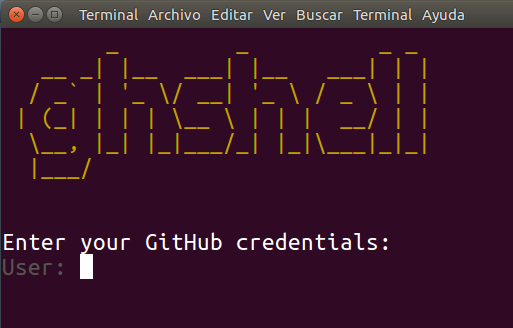
\includegraphics[width=0.7\textwidth]{images/ghshell1}
		\caption{Login de usuario}
		\label{fig:ghshell1}
		\end{center}
		\end{figure}
		
 
 		\begin{figure}[H]
		\begin{center}
		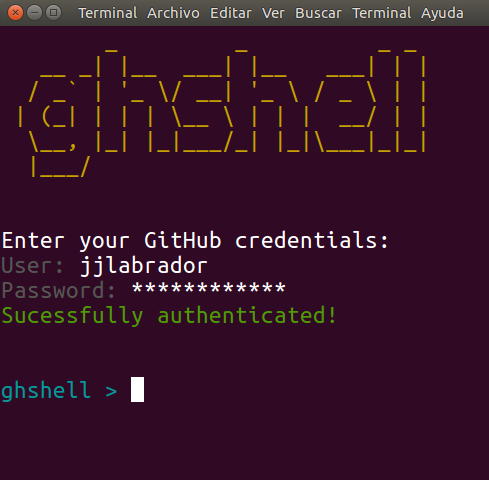
\includegraphics[width=0.6\textwidth]{images/ghshell2-1}
		\caption{Usuario autenticado}
		\label{fig:ghshell2-1}
		\end{center}
		\end{figure}
		
    Una vez que el usuario se autentifica con GitHub, se genera un token personal, que se usa posteriormente para acceder a la API de Github. Este token se almacena cifrado en el equipo del usuario, por lo que las siguientes ocasiones que utilice la herramienta no hará falta que vuelva a iniciar sesión:
        
        \begin{figure}[H]
		\begin{center}
		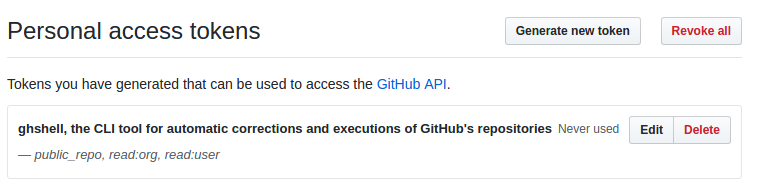
\includegraphics[width=1\textwidth]{images/ghshell2-3}
		\caption{Token personal en GitHub}
		\label{fig:ghshell2-3}
		\end{center}
		\end{figure}
		
		\begin{figure}[H]
		\begin{center}
		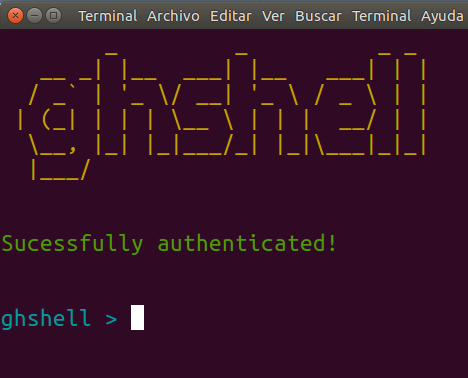
\includegraphics[width=0.6\textwidth]{images/ghshell2-4}
		\caption{Login automático una vez generado el token}
		\label{fig:ghshell2-4}
		\end{center}
		\end{figure}
		
	Si el usuario cierra sesión en la herramienta, se eliminará el token en GitHub y en el equipo:
	
		\begin{figure}[H]
		\begin{center}
		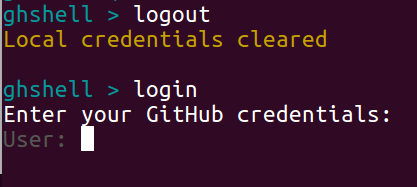
\includegraphics[width=0.6\textwidth]{images/ghshell2-2}
		\caption{Logout de usuario}
		\label{fig:ghshell2-2}
		\end{center}
		\end{figure}
		
\newpage
%---------------------------------------------------------------------------------

\subsection{Contexto principal}
\label{subsec:b.2.2}

	Una vez autentificados, en el menú principal podremos hacer las siguientes acciones:
	
	\begin{itemize}
		\item \underline{Mostrar la ayuda}. Comando \verb|help|.
		
		\begin{verbatim}
			ghshell > help
		\end{verbatim}
		
		En función del contexto donde nos encontremos, se mostrarán diferentes opciones en la ayuda.
		
		\begin{figure}[H]
		\begin{center}
		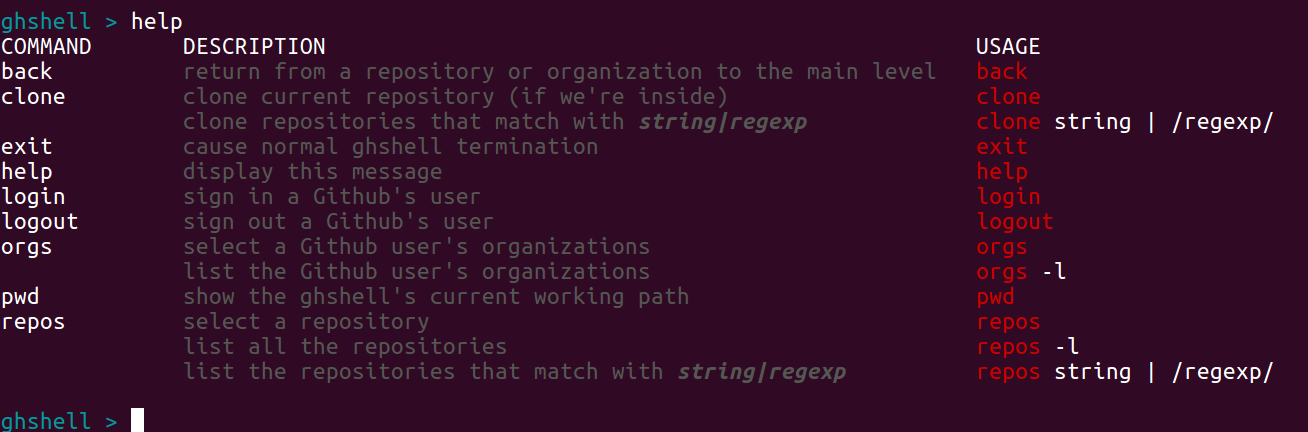
\includegraphics[width=1\textwidth]{images/help1-1}
		\caption{Ayuda global}
		\label{fig:help1-1}
		\end{center}
		\end{figure}
		
		%-------------------
		\item \underline{Mostrar el directorio de trabajo actual}. Comando \verb|pwd|.
		
		\begin{verbatim}
			ghshell > pwd
		\end{verbatim}
		
		Visualiza el directorio de trabajo donde se ha ejecutado el programa:
		
		\begin{figure}[H]
		\begin{center}
		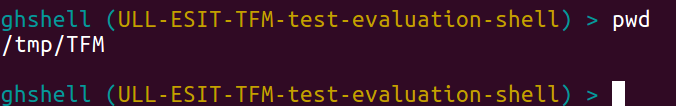
\includegraphics[width=0.7\textwidth]{images/pwd}
		\caption{Directorio actual de trabajo}
		\label{fig:pwd}
		\end{center}
		\end{figure}
		
		{\bfseries NOTA}: este comando tiene el mismo comportamiento si nos encontramos dentro de una organización o dentro de un repositorio de una organización.
		\newpage
		
		%-------------------
		\item  \underline{Listar y acceder a organizaciones}. Comando \verb|orgs|.
		
		\begin{verbatim}
			ghshell > orgs [-l]
		\end{verbatim}
		
		Si se ejecuta el comando sin argumentos, pregunta al usuario a qué organización quiere acceder. Se puede usar la tecla tabulador para ver las organizaciones disponibles.
		
		\begin{figure}[H]
		\begin{center}
		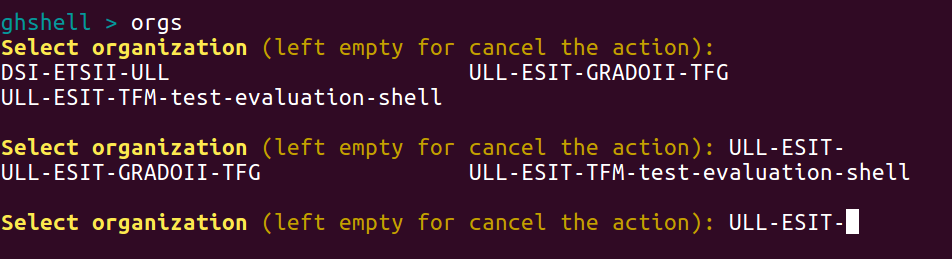
\includegraphics[width=0.8\textwidth]{images/orgs1-1}
		\caption{Acceso a una organización}
		\label{fig:orgs1-1}
		\end{center}
		\end{figure}
		
		El {\it prompt} de la consola cambiará para indicarnos que nos encontramos dentro de la organización.
		\bigskip
		
		Si se ejecuta el comando con la opción \verb|-l|, simplemente lista las organizaciones a las que pertenece el usuario.
		
		\begin{figure}[H]
		\begin{center}
		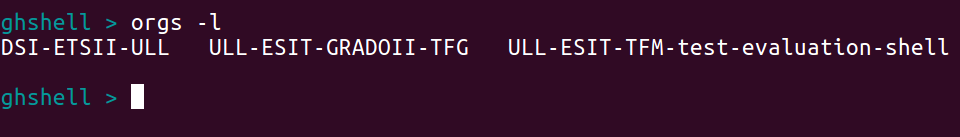
\includegraphics[width=0.8\textwidth]{images/ghshell3}
		\caption{Lista de organizaciones del usuario}
		\label{fig:ghshell3}
		\end{center}
		\end{figure}

\newpage
		%-------------------
		\item  \underline{Listar y acceder a repositorios}. Comando \verb|repos|.
		
		\begin{verbatim}
			ghshell > repos [-l] [string | /regexp/]
		\end{verbatim}
		
		Si se ejecuta el comando sin argumentos, pregunta al usuario a qué repositorio quiere acceder. Se puede usar la tecla tabulador para ver los repositorios disponibles.
		
		\begin{figure}[H]
		\begin{center}
		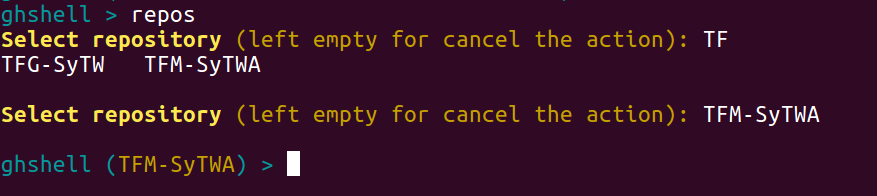
\includegraphics[width=0.8\textwidth]{images/repos1-1}
		\caption{Acceso a un repositorio}
		\label{fig:repos1-1}
		\end{center}
		\end{figure}
		
		
		El {\it prompt} de la consola cambiará para indicarnos que nos encontramos dentro de un repositorio.		
		\bigskip
		
		Si se ejecuta el comando con la opción \verb|-l|, simplemente se listan los repositorios que pertenecen al usuario.
		
		\begin{figure}[H]
		\begin{center}
		\includegraphics[width=1\textwidth]{images/repos1-2}
		\caption{Listado de repositorios del usuario}
		\label{fig:repos1-2}
		\end{center}
		\end{figure}

\newpage
	
		Si se especifica como argumento un string o expresión regular, se mostrarán los repositorios que coincidan con ese argumento:
		
		\begin{figure}[H]
		\begin{center}
		\includegraphics[width=0.4\textwidth]{images/repos1-3}
		\caption{Listado de repositorios del usuario que coinciden con el argumento pasado}
		\label{fig:repos1-3}
		\end{center}
		\end{figure}
		
		
		{\bfseries NOTA}: este comando tiene el mismo comportamiento si nos encontramos dentro de una organización:
		
		
		\begin{figure}[H]
		\begin{center}
		\includegraphics[width=0.9\textwidth]{images/repos1-4}
		\caption{Acceso a un repositorio dentro de una organización}
		\label{fig:repos1-4}
		\end{center}
		\end{figure}
		
		\begin{figure}[H]
		\begin{center}
		\includegraphics[width=1\textwidth]{images/repos1-5}
		\caption{Listado de repositorios de una organización}
		\label{fig:repos1-5}
		\end{center}
		\end{figure}
		
		\begin{figure}[H]
		\begin{center}
		\includegraphics[width=0.7\textwidth]{images/repos1-6}
		\caption{Listado de repositorios de una organización que coinciden con el argumento pasado}
		\label{fig:repos1-6}
		\end{center}
		\end{figure}	
		
		%-------------------
		\item  \underline{Clonar repositorios}. Comando \verb|clone|.
		
		\begin{verbatim}
			ghshell > clone string | /regexp/
		\end{verbatim}	
		
		Al especificar el argumento como un string o expresión regular, se clonarán todos los repositorios que coincidan con ese argumento. 
		
		\begin{figure}[H]
		\begin{center}
		\includegraphics[width=0.9\textwidth]{images/clone1-1}
		\caption{Clonado de repositorios que coinciden con el string pasado}
		\label{fig:clone1-1}
		\end{center}
		\end{figure}
		
		\begin{figure}[H]
		\begin{center}
		\includegraphics[width=0.9\textwidth]{images/clone1-2}
		\caption{Clonado de repositorios que coinciden con la regexp pasada}
		\label{fig:clone1-2}
		\end{center}
		\end{figure}
		
		
		El clonado se realiza de manera {\bfseries asíncrona}, por lo que podemos seguir trabajando mientras se clona(n) el/los repositorio(s). 
\bigskip
		
		Se puede observar el estado de la clonación revisando el fichero de log que se genera: \textless \verb|nombre-repositorio|\textgreater \verb|-clone.log|.:
		
		\begin{figure}[H]
		\begin{center}
		\includegraphics[width=0.7\textwidth]{images/clone1-3}
		\caption{Resultado del clonado de repositorios}
		\label{fig:clone1-3}
		\end{center}
		\end{figure}
		
\newpage		
		Los fichero de log muestran la información del clonado. Se ha añadido una huella de tiempo para tener un control más exacto sobre cuándo ocurre cada evento:
		
		\begin{verbatim}
[2017/07/02-01:20:47] Clonar en «TFM-SyTWA»...

[2017/07/02-01:20:48] remote: Counting objects: 92, done.        

[2017/07/02-01:20:48] remote: Compressing objects:   1% (1/65)           
remote: Compressing objects:   3% (2/65)           
remote: Compressing objects:   4% (3/65)           
remote: Compressing objects:   6% (4/65)           
remote: Compressing objects:   7% (5/65)           
remote: Compressing objects:   9% (6/65)           
remote: Compressing objects:  10% (7/65)           
remote: Compressing objects:  12% (8/65)           
remote: Compressing objects:  13% (9/65)           
remote: Compressing objects:  15% (10/65)           
remote: Compressing objects:  16% (11/65)           
remote: Compressing objects:  18% (12/65)           
[2017/07/02-01:20:48] remote: Compressing objects:  20% (13/65)           
remote: Compressing objects:  21% (14/65)           
remote: Compressing objects:  23% (15/65)           
remote: Compressing objects:  24% (16/65)           
remote: Compressing objects:  26% (17/65)           
remote: Compressing objects:  27% (18/65)           
remote: Compressing objects:  29% (19/65)           
remote: Compressing objects:  30% (20/65)           
remote: Compressing objects:  32% (21/65)           
remote: Compressing objects:  33% (22/65)           
remote: Compressing objects:  35% (23/65)           
remote: Compressing objects:  36% (24/65)           
remote: Compressing objects:  38% (25/65)           
remote: Compressing objects:  40% (26/65)           
remote: Compressing objects:  41% (27/65)           
remote: Compressing objects:  43% (28/65)           
remote: Compressing objects:  44% (29/65)           
remote: Compressing objects:  46% (30/65)           
remote: Compressing objects:  47% (31/65)           
remote: Compressing objects:  49% (32/65)           
remote: Compressing objects:  50% (33/65)           
remote: Compressing objects:  52% (34/65)           
remote: Compressing objects:  53% (35/65)           
remote: Compressing objects:  55% (36/65)           
remote: Compressing objects:  56% (37/65)           
remote: Compressing objects:  58% (38/65)           
remote: Compressing objects:  60% (39/65)           
remote: Compressing objects:  61% (40/65)           
remote: Compressing objects:  63% (41/65)           
remote: Compressing objects:  64% (42/65)           
remote: Compressing objects:  66% (43/65)           
remote: Compressing objects:  67% (44/65)           
remote: Compressing objects:  69% (45/65)           
remote: Compressing objects:  70% (46/65)           
remote: Compressing objects:  72% (47/65)           
remote: Compressing objects:  73% (48/65)           
remote: Compressing objects:  75% (49/65)           
remote: Compressing objects:  76% (50/65)           
remote: Compressing objects:  78% (51/65)           
remote: Compressing objects:  80% (52/65)           
remote: Compressing objects:  81% (53/65)           
remote: Compressing objects:  83% (54/65)           
remote: Compressing objects:  84% (55/65)           
remote: Compressing objects:  86% (56/65)           
remote: Compressing objects:  87% (57/65)           
remote: Compressing objects:  89% (58/65)           
remote: Compressing objects:  90% (59/65)           
remote: Compressing objects:  92% (60/65)           
remote: Compressing objects:  93% (61/65)           
remote: Compressing objects:  95% (62/65)           
remote: Compressing objects:  96% (63/65)           
remote: Compressing objects:  98% (64/65)           
remote: Compressing objects: 100% (65/65)           
remote: Compressing objects: 100% (65/65), done.        

[2017/07/02-01:20:49] remote: Total 92 (delta 25), reused 92 (delta 25), pack-reused 0        

[2017/07/02-01:20:49] Comprobando la conectividad… 
[2017/07/02-01:20:49] hecho.

\end{verbatim}

\newpage		
		%-------------------		
		\item  \underline{Salir del programa}. Comando \verb|exit|.
		
		\bigskip
		Causa el cierre ordenado del programa.
		\bigskip
				
		{\bfseries NOTA}: este comando tiene el mismo comportamiento si nos encontramos dentro de una organización o dentro de un repositorio de una organización. 
		
	\end{itemize}

\subsection{Contexto de organización}
\label{subsec:b.2.2}

	Los comandos \verb|pwd|, \verb|repos|, \verb|clone| y \verb|exit| tienen el mismo comportamiento que en el contexto principal. 
\bigskip

	Además, en el caso del comando \verb|clone|, se creará una carpeta con el nombre de la organización en la que nos encontremos y en ella se guardarán todos los repositorios clonados.
	
	%-------------------
\begin{itemize}

	\item \underline{Mostrar la ayuda}. Comando \verb|help|.
		
		\begin{verbatim}
			ghshell > help
		\end{verbatim}
		
		En función del contexto donde nos encontremos, se mostrarán diferentes opciones en la ayuda.
		
		\begin{figure}[H]
		\begin{center}
		\includegraphics[width=1\textwidth]{images/help1-2}
		\caption{Ayuda en el contexto de organización}
		\label{fig:help1-2}
		\end{center}
		\end{figure}

\newpage	
	%-------------------	
	\item \underline{Salir del contexto actual}. Comando \verb|back|.
	
		\begin{verbatim}
			ghshell > back
		\end{verbatim}
		
		Si nos encontramos en un repositorio propio o en una organización, regresamos al contexto principal. 
		Si nos encontramos dentro de un repositorio de una organización, regresamos al contexto de la organización.
		
		\begin{figure}[H]
		\begin{center}
		\includegraphics[width=0.7\textwidth]{images/back1-1}
		\caption{Regreso al contexto principal desde una organización}
		\label{fig:back1-1}
		\end{center}
		\end{figure}
		
		\begin{figure}[H]
		\begin{center}
		\includegraphics[width=0.8\textwidth]{images/back1-2}
		\caption{Regreso al contexto principal desde un repositorio}
		\label{fig:back1-2}
		\end{center}
		\end{figure}
		
	%-------------------	
	\item \underline{Ejecutar un script determinado}. Comando \verb|script|.
	
		\begin{verbatim}
			ghshell > script <file> /regexp/
		\end{verbatim}
		
	Este comando sirve para ejecutar un script. La ruta del fichero del script puede ser absoluta o relativa.
\bigskip

	El script debe estar escrito en \verb|Bash|.	
	
	
	Al especificar una expresión regular, se ejecutará el script en todos los repositorios que coincidan con la expresión regular indicada.
	
		\begin{figure}[H]
		\begin{center}
		\includegraphics[width=0.8\textwidth]{images/script1-1}
		\caption{Ejecución de script en repositorios que coinciden con la regexp pasada}
		\label{fig:script1-1}
		\end{center}
		\end{figure}
		
\newpage
	
	La ejecución de cada script se ejecuta en un proceso hijo independiente pero, a diferencia del clonado, el script se ejecuta línea a línea de manera {\bfseries síncrona}. 
\bigskip
	
	Se puede observar el estado de la ejecución del script y los resultados revisando el fichero de log que se genera:
	\bigskip
	\textless \verb|nombre-repositorio|\textgreater \verb|-|\textless \verb|nombre-script|\textgreater \verb|.log|
	
		\begin{figure}[H]
		\begin{center}
		\includegraphics[width=0.7\textwidth]{images/script1-2}
		\caption{Fichero de log generado resultante de la ejecución del script}
		\label{fig:script1-2}
		\end{center}
		\end{figure}
	
	%-------------------
	\item \underline{Exportar resultados}. Comando \verb|book|.
	
		\begin{verbatim}
			ghshell > book string | /regexp/
		\end{verbatim}
	
	Este comando genera un {\bfseries Gitbook} con los resultados de todos los scripts ejecutados sobre los repositorios. Este libro se genera en formato PDF y en HTML.
\bigskip
	
	Al especificar un string o expresión regular, se creará el libro por cada repositorios que coincida con la expresión regular indicada.
	
		\begin{figure}[H]
		\begin{center}
		\includegraphics[width=0.8\textwidth]{images/book1-1}
		\caption{Creación del Gitbook en repositorios que coinciden con la regexp pasada}
		\label{fig:book1-1}
		\end{center}
		\end{figure}
		
	
	La creación del libro se realiza de manera {\bfseries asíncrona}, por lo que se puede seguir trabajando mientras se genera. 
\bigskip
	
	Se puede observar el estado de la creación del libro y su exportación a PDF revisando los ficheros de logs que se generan:
\bigskip

	\textless \verb|nombre-repositorio|\textgreater \verb|-gitbook_build.out| y 
\bigskip
	
	\textless \verb|nombre-repositorio|\textgreater \verb|-gitbook_pdf.out|.
	\bigskip
	\bigskip
	
	Tanto el PDF como el HTML contará con las siguientes páginas:
		
		\begin{itemize}
			\item Índice (Tabla de contenidos).
			\item Introducción: en esta página se copiará el fichero {\it README.md} del repositorio. En caso de que no tuviera ese fichero, se imprimirá un mensaje que indica que el repositorio no tiene fichero README.md.
			\item Páginas correspondientes a la ejecución de cada script.
		\end{itemize}
		
		
    La carpeta que contiene el libro en HTML se llamará:
    \bigskip
     
	\textless \verb|nombre-repositorio|\textgreater \verb|_gitbook/_book|. 
		
		\begin{figure}[H]
		\begin{center}
		\includegraphics[width=0.7\textwidth]{images/ghshell8-4}
		\caption{Localización del HTML del Gitbook}
		\label{fig:ghshell8-4}
		\end{center}
		\end{figure}

\bigskip

	Para visualizar el libro en formato HTML, basta con ejecutar el comando:
	
	\begin{verbatim}
		[~]$ gitbook serve
	\end{verbatim}
	
	Se arrancará un servidor web y, accediendo a la página que nos indique la consola, se podrá leer el libro:
	
		\begin{figure}[H]
		\begin{center}
		\includegraphics[width=0.9\textwidth]{images/ghshell8-5}
		\caption{Visualizar libro en HTML (I)}
		\label{fig:ghshell8-5}
		\end{center}
		\end{figure}
		
		\begin{figure}[H]
		\begin{center}
		\includegraphics[width=0.7\textwidth]{images/ghshell8-10}
		\caption{Visualizar libro en HTML (II)}
		\label{fig:ghshell8-10}
		\end{center}
		\end{figure}

\newpage		
		
	El fichero PDF generado se llamará \textless \verb|nombre-repositorio|\textgreater \verb|.pdf|. 
	
        \begin{figure}[H]
		\begin{center}
		\includegraphics[width=0.9\textwidth]{images/ghshell8-6}
		\caption{Indice del PDF generado}
		\label{fig:ghshell8-6}
		\end{center}
		\end{figure}
		
		\begin{figure}[H]
		\begin{center}
		\includegraphics[width=0.7\textwidth]{images/ghshell8-7}
		\caption{Introducción del PDF generado}
		\label{fig:ghshell8-7}
		\end{center}
		\end{figure}
		
		\begin{figure}[H]
		\begin{center}
		\includegraphics[width=0.7\textwidth]{images/ghshell8-8}
		\caption{Resultado del clonado del repositorio}
		\label{fig:ghshell8-8}
		\end{center}
		\end{figure}
		
		\begin{figure}[H]
		\begin{center}
		\includegraphics[width=0.7\textwidth]{images/ghshell8-9}
		\caption{Resultado de la ejecución del script en el repositorio}
		\label{fig:ghshell8-9}
		\end{center}
		\end{figure}   
	
	
	
\newpage
	
	%-------------------	 
	\item \underline{Seleccionar assignments}. Comando \verb|assignments|.
	
		\begin{verbatim}
			ghshell > assignments string | /regexp/ [clone|book|script <file>]
		\end{verbatim}
		
		Los assignments son tratados como un caso especial de repositorios dentro de una organización.
		
		Si sólo se pasa como argumento un string o una expresión regular, listará los assignments que coincidan con dicho argumento.
		
		\begin{figure}[H]
		\begin{center}
		\includegraphics[width=0.8\textwidth]{images/assignments1-1}
		\caption{Assignments que coinciden con la expresión regular}
		\label{fig:assignment1-1}
		\end{center}
		\end{figure}
		
		
		En el caso de que además se pase alguno de los parámetros: \verb|clone|, \verb|script <file>| o \verb|book|; se clonará, se ejecutará un script o se creará un libro respectivamente en los repositorios que coincidan con el string o la expresión regular. 
\bigskip

Además, en el caso del comando \verb|clone|, se creará una carpeta con el nombre de la asignación que contendrá todas las asignaciones clonadas.
	
		\begin{figure}[H]
		\begin{center}
		\includegraphics[width=1\textwidth]{images/ghshell6-1}
		\caption{Clonado de asignaciones que coinciden con la expresión regular}
		\label{fig:ghshell6-1}
		\end{center}
		\end{figure}
		
		\begin{figure}[H]
		\begin{center}
		\includegraphics[width=1\textwidth]{images/assignments1-2}
		\caption{Ejecución de script en assignments que coinciden con la expresión regular}
		\label{fig:assignment1-2}
		\end{center}
		\end{figure}
		
		\begin{figure}[H]
		\begin{center}
		\includegraphics[width=1\textwidth]{images/assignments1-3}
		\caption{Creación del Gitbook en los assignments que coinciden con la expresión regular}
		\label{fig:assignment1-3}
		\end{center}
		\end{figure}
		
		\begin{figure}[H]
		\begin{center}
		\includegraphics[width=0.8\textwidth]{images/assignments1-4}
		\caption{Directorios y ficheros generados}
		\label{fig:assignment1-4}
		\end{center}
		\end{figure}		
	
\end{itemize}
\newpage

\subsection{Contexto de repositorio}
\label{subsec:b.2.3}

	Los comandos \verb|pwd| y \verb|exit| tienen el mismo comportamiento que en el contexto principal. 
\bigskip
	
	El comando \verb|back| tienen el mismo comportamiento que en el contexto de organizaciones.
	
\begin{itemize}

	\item \underline{Mostrar la ayuda}. Comando \verb|help|.
		
		\begin{verbatim}
			ghshell > help
		\end{verbatim}
		
		En función del contexto donde nos encontremos, se mostrarán diferentes opciones en la ayuda.
				
		\begin{figure}[H]
		\begin{center}
		\includegraphics[width=1\textwidth]{images/help1-3}
		\caption{Ayuda en el contexto de un repositorio}
		\label{fig:help1-2}
		\end{center}
		\end{figure}

	%-------------------	
	\item \underline{Clonar repositorios}. Comando \verb|clone|.
	
		\begin{verbatim}
			ghshell > clone
		\end{verbatim}
		
		En este contexto, se ejecuta sin argumentos y clona el repositorio donde nos encontremos.
		
		\begin{figure}[H]
		\begin{center}
		\includegraphics[width=1\textwidth]{images/clone1-4}
		\caption{Clonado de un repositorio dentro de una organización}
		\label{fig:clone1-4}
		\end{center}
		\end{figure}

\newpage
	
	%-------------------		
	\item \underline{Ejecutar un script determinado}. Comando \verb|script|.
	
		\begin{verbatim}
			ghshell > script <file>
		\end{verbatim}
		
		En este contexto, se ejecuta sin argumentos y ejecuta el script indicado sobre el repositorio donde nos encontremos.
		
		\begin{figure}[H]
		\begin{center}
		\includegraphics[width=1\textwidth]{images/script1-3}
		\caption{Ejecución de un script en un repositorio dentro de una organización}
		\label{fig:script1-3}
		\end{center}
		\end{figure}
		
	%-------------------
	\item \underline{Exportar resultados}. Comando \verb|book|.
	
		\begin{verbatim}
			ghshell > book
		\end{verbatim}
		
		En este contexto, se ejecuta sin argumentos y crea un Gitbook con los resultados de todos los scripts ejecutados sobre el repositorio donde nos encontremos.
		
		\begin{figure}[H]
		\begin{center}
		\includegraphics[width=1\textwidth]{images/book1-3}
		\caption{Creación del Gitbook en un repositorio dentro de una organización}
		\label{fig:book1-3}
		\end{center}
		\end{figure}
	
	%-------------------	
	\item \underline{Obtener el propietario del repositorio}. Comando \verb|owner|.
	
		\begin{verbatim}
			ghshell > owner
		\end{verbatim}
		
		\begin{figure}[H]
		\begin{center}
		\includegraphics[width=0.5\textwidth]{images/owner1-1}
		\caption{Propietario del repositorio}
		\label{fig:owner1-1}
		\end{center}
		\end{figure}
		
		Además, si nos encontramos en un repositorio que pertenece a una organización, muestra también los contribuyentes.
		
		\begin{figure}[H]
		\begin{center}
		\includegraphics[width=1\textwidth]{images/owner1-2}
		\caption{Contribuyentes del repositorio}
		\label{fig:owner1-2}
		\end{center}
		\end{figure}
	
\end{itemize}





\end{appendix}

%%%%%%%%%%%%%%%%%%%%%%%%%%%%%%%%%%%%%%%%%%%%%%%%%%%%%%%%%%%%%%%%%%%%%%%%%%%%%%%
\clearpage
\phantomsection

\addcontentsline{toc}{chapter}{Índice alfabético}
\printindex

%%%%%%%%%%%%%%%%%%%%%%%%%%%%%%%%%%%%%%%%%%%%%%%%%%%%%%%%%%%%%%%%%%%%%%%%%%%%%%%
\addcontentsline{toc}{chapter}{Bibliografía}
\bibliographystyle{plain}%{ieeetr}

\bibliography{TFM}
\nocite{*}

%%%%%%%%%%%%%%%%%%%%%%%%%%%%%%%%%%%%%%%%%%%%%%%%%%%%%%%%%%%%%%%%%%%%%%%%%%%%%%%

\end{document}
